\chapter{Interfejs użytkownika}

Zrzuty ekranu wykonano w~przeglądarce Chrome przy szerokości 1440 px (o ile nie podano
inaczej) na danych demonstracyjnych z~polecenia \code{seed\_demo}. Uczeń: konto
\code{student1}, nauczyciel: \code{instructor}, administrator: \code{admin}
(motyw ciemny ,,Ocean'' wybrany w~jego profilu).

\section{Przepływ nawigacji}

\begin{figure}[H]
\centering
\resizebox{\linewidth}{!}{%
\begin{tikzpicture}[node distance=0.5cm and 0.6cm]
  \tikzset{pg/.style={box,minimum width=2.4cm,text width=2.3cm,minimum height=0.7cm}}
  \node[pg,fill=paperdark] (home) {Strona główna};
  \node[pg,right=of home] (cat) {Katalog};
  \node[pg,right=of cat] (course) {Kurs};
  \node[pg,right=of course] (lesson) {Lekcja / test};
  \node[pg,right=of lesson] (res) {Wynik, dyplom};
  \node[pg,below=of course] (cart) {Koszyk};
  \node[pg,right=of cart] (chk) {Zamówienie};
  \node[pg,right=of chk] (stripe) {Stripe};
  \node[pg,below=of home] (login) {Logowanie / rejestracja};
  \node[pg,below=of login] (prof) {Profil, motywy};
  \node[pg,below=of cat] (gal) {Galeria};
  \node[pg,below=of gal] (notif) {Powiadomienia};
  \node[pg,below=of cart] (mod) {Moderacja (zakładki)};
  \node[pg,right=of mod] (create) {Kreator kursu};
  \node[pg,right=of create] (my) {Moje kursy};
  \draw[arr] (home) -- (cat); \draw[arr] (cat) -- (course); \draw[arr] (course) -- (lesson); \draw[arr] (lesson) -- (res);
  \draw[arr] (course) -- (cart); \draw[arr] (cart) -- (chk); \draw[arr] (chk) -- (stripe);
  \draw[arr] (stripe.north) -- (lesson.south);
  \draw[arr] (home) -- (login); \draw[arr] (login) -- (prof);
  \draw[arr] (home.south east) -- (gal.north west);
  \draw[arr] (my) -- (lesson.south east);
  \draw[arr] (create) -- (my);
  \draw[arr] (mod) -- (create);
\end{tikzpicture}}
\caption{Główne ścieżki nawigacji (nagłówek z~menu jest dostępny na każdej stronie)}
\end{figure}

Dostęp do stron chronionych sprawdza serwer: niezalogowany użytkownik jest przekierowany
na logowanie z~parametrem \code{next}, a~po zalogowaniu wraca na żądaną stronę. Pozycje
menu zależą od roli (np.\ ,,Moderacja'' i~,,Utwórz kurs'' dla nauczyciela, ,,Zaproponuj
kurs'' dla ucznia), ale sam brak linku nigdy nie jest jedynym zabezpieczeniem.

\section{Strona główna i~nawigacja}

\begin{figure}[H]
\centering
\fcolorbox{rule}{white}{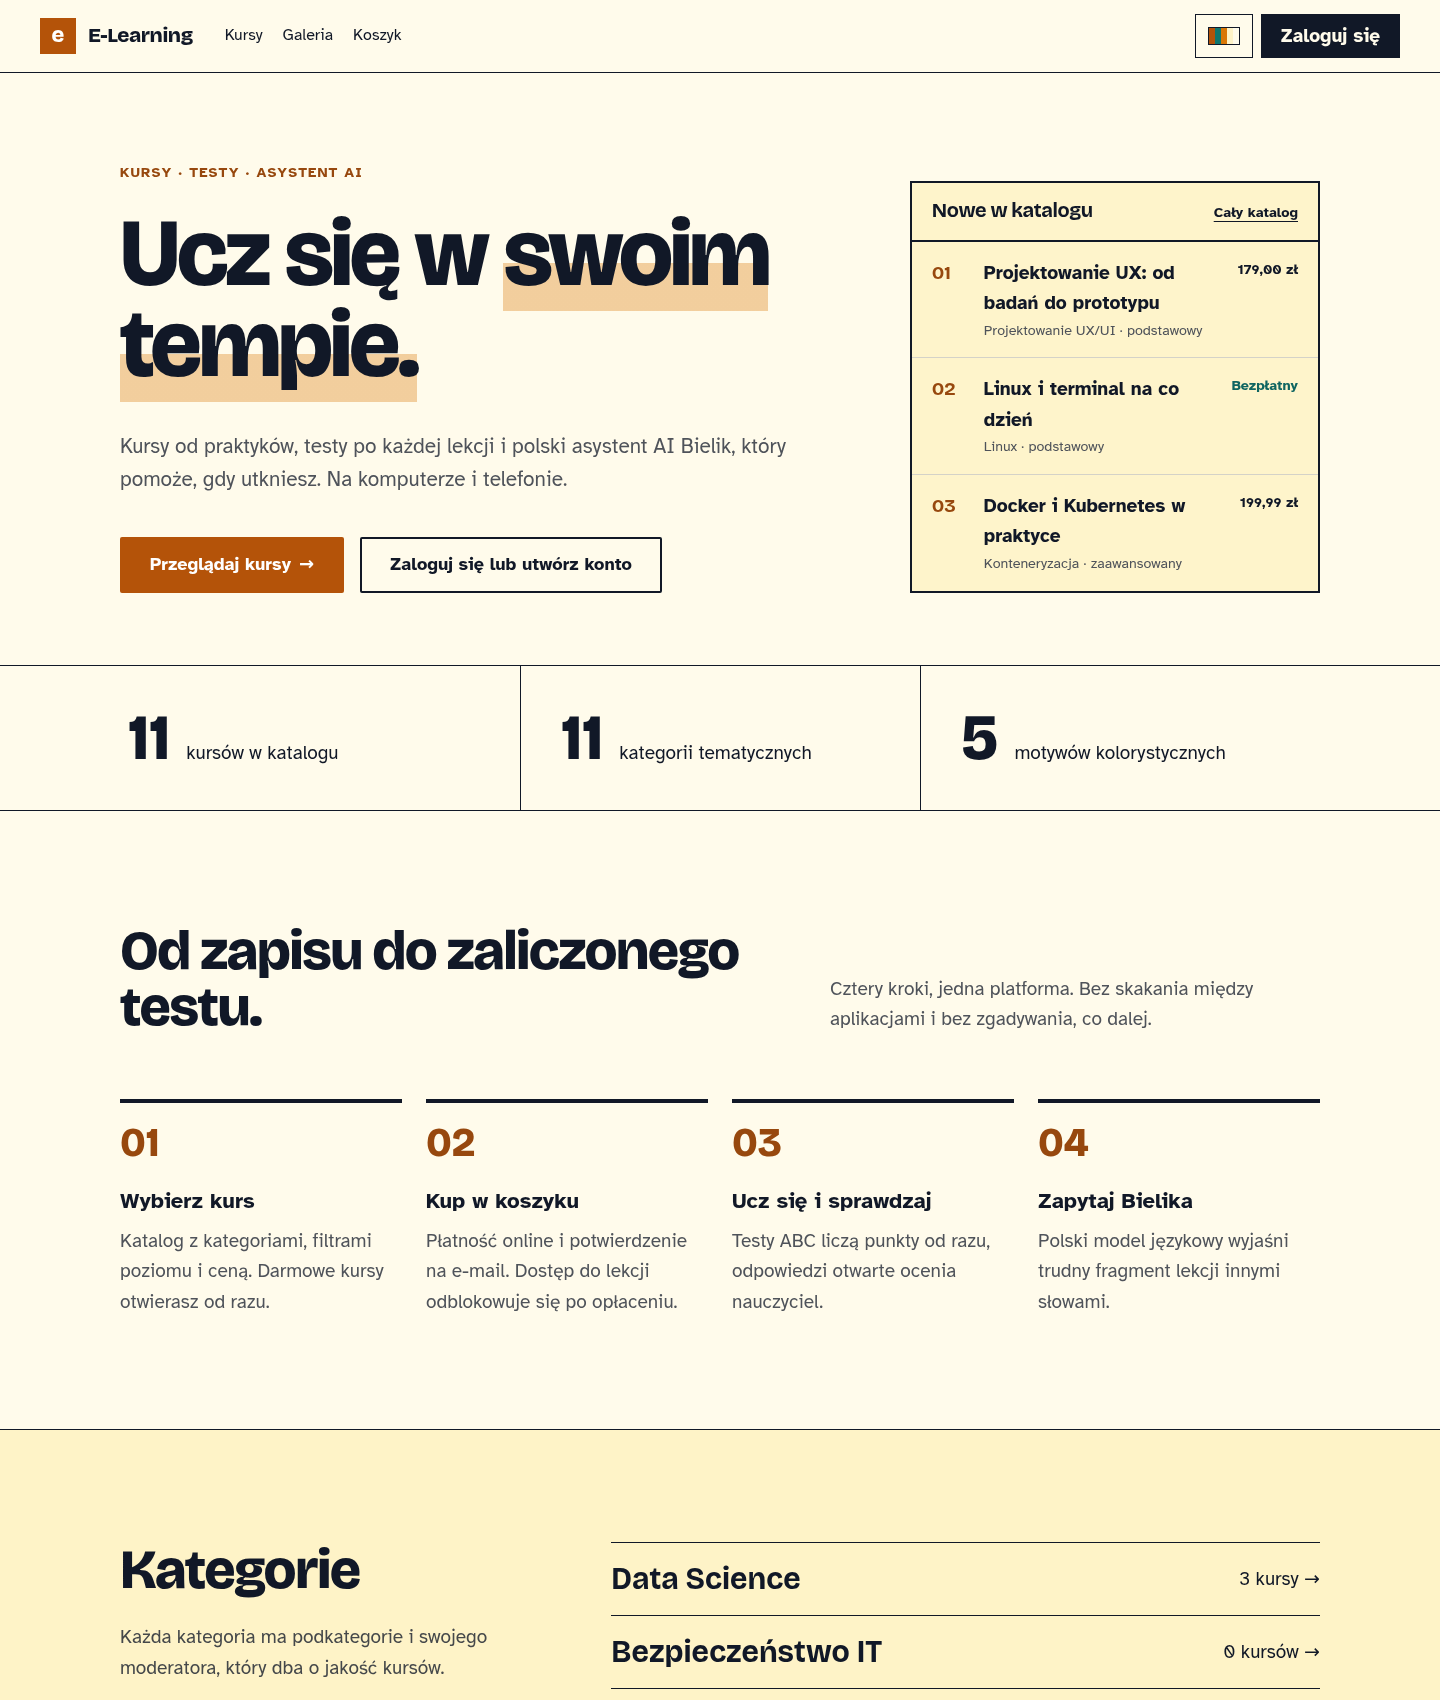
\includegraphics[width=0.94\linewidth,height=0.37\textheight,keepaspectratio]{img/home.png}}
\caption{Strona główna (gość, motyw domyślny ,,Bursztyn'')}\label{fig:ui-home}
\end{figure}
Nagłówek zawiera logo, menu główne, przełącznik motywu i~przycisk logowania. Pod sekcją powitalną widać najnowsze kursy z~bazy, prawdziwe liczby (kursy, kategorie, motywy), cztery numerowane kroki i~listę kategorii z~licznikami.


\begin{figure}[H]
\centering
\fcolorbox{rule}{white}{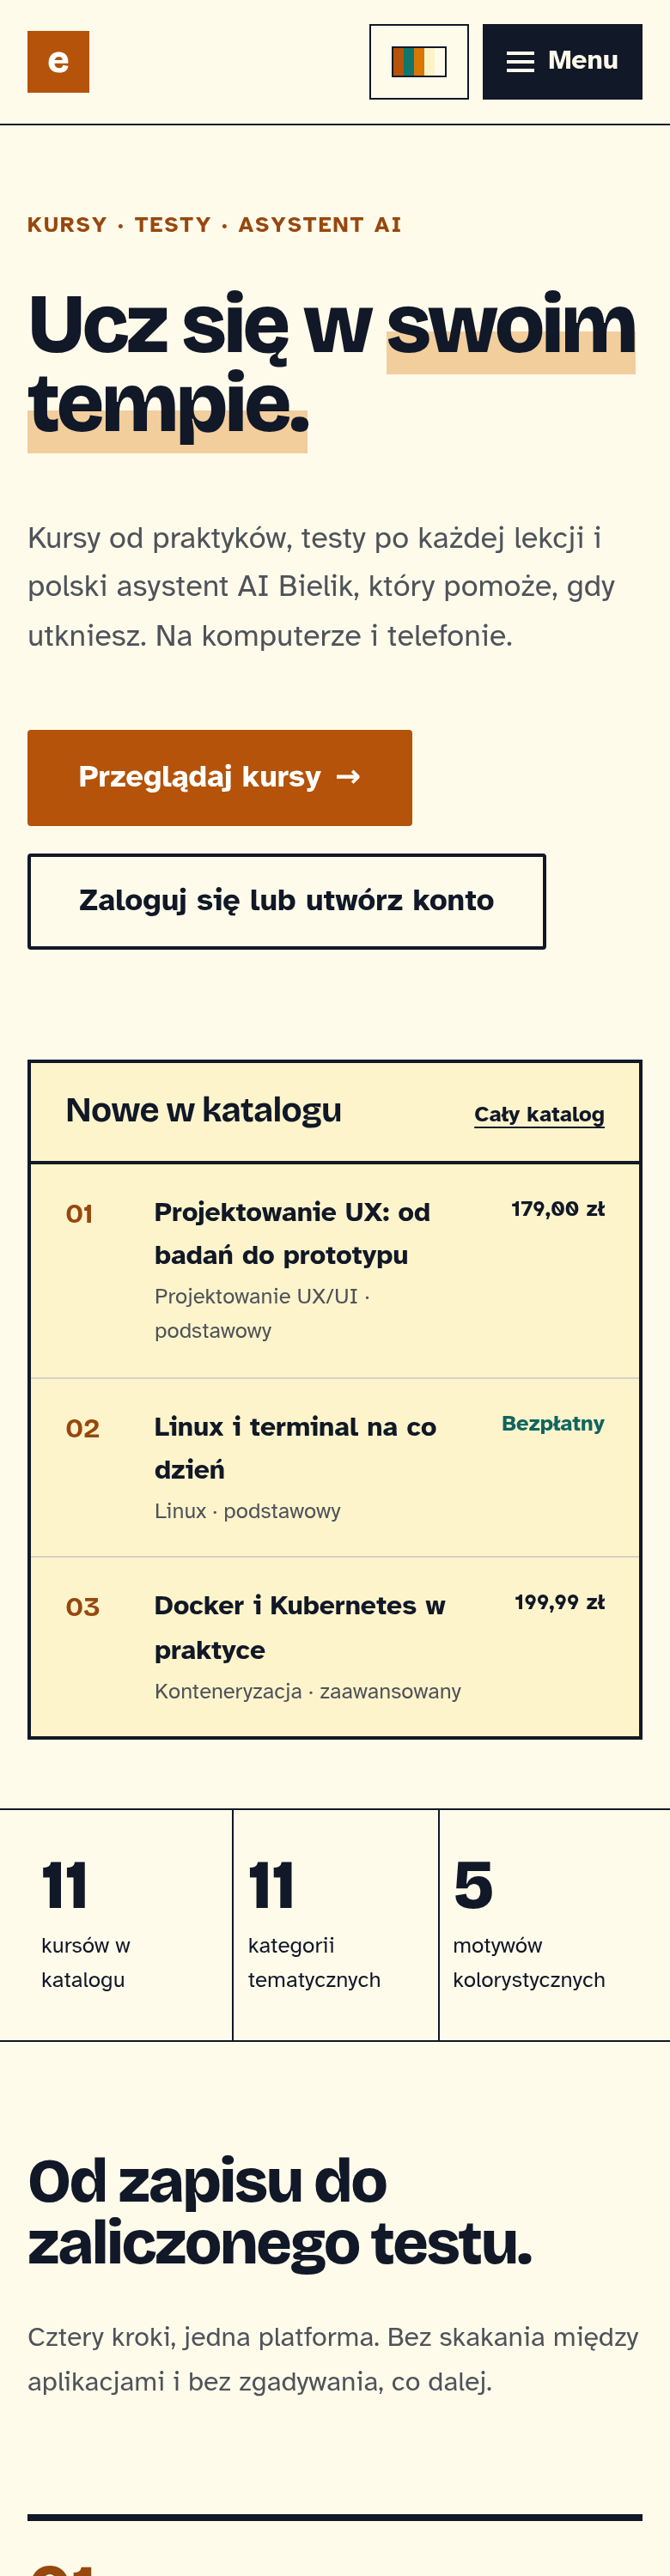
\includegraphics[width=0.94\linewidth,height=0.42\textheight,keepaspectratio]{img/home_mobile.png}}
\caption{Strona główna na telefonie (390 px)}\label{fig:ui-home-mobile}
\end{figure}
Menu zwija się do przycisku ,,Menu'', siatki przechodzą w~jedną kolumnę, nie pojawia się poziomy pasek przewijania.


\section{Konto}

\begin{figure}[H]
\centering
\fcolorbox{rule}{white}{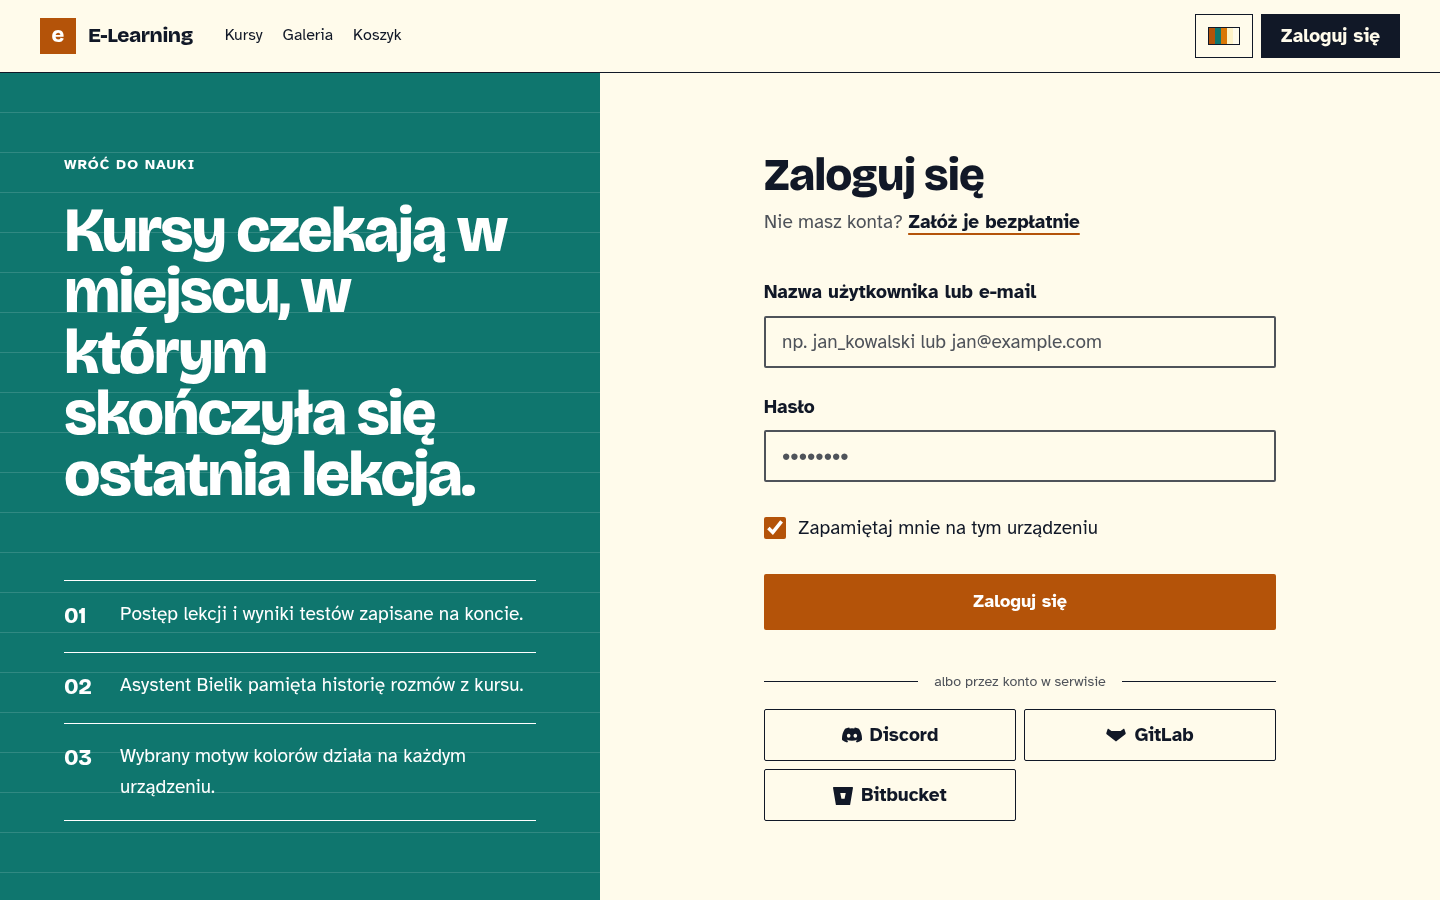
\includegraphics[width=0.94\linewidth,height=0.37\textheight,keepaspectratio]{img/login.png}}
\caption{Logowanie -- układ split-screen}\label{fig:ui-login}
\end{figure}
Na komputerze panel informacyjny stoi obok formularza (asymetrycznie), a~pod formularzem są przyciski portali Discord, GitLab i~Bitbucket. Każde pole ma etykietę, a~,,Zapamiętaj mnie'' to zwykłe pole wyboru.


\begin{figure}[H]
\centering
\fcolorbox{rule}{white}{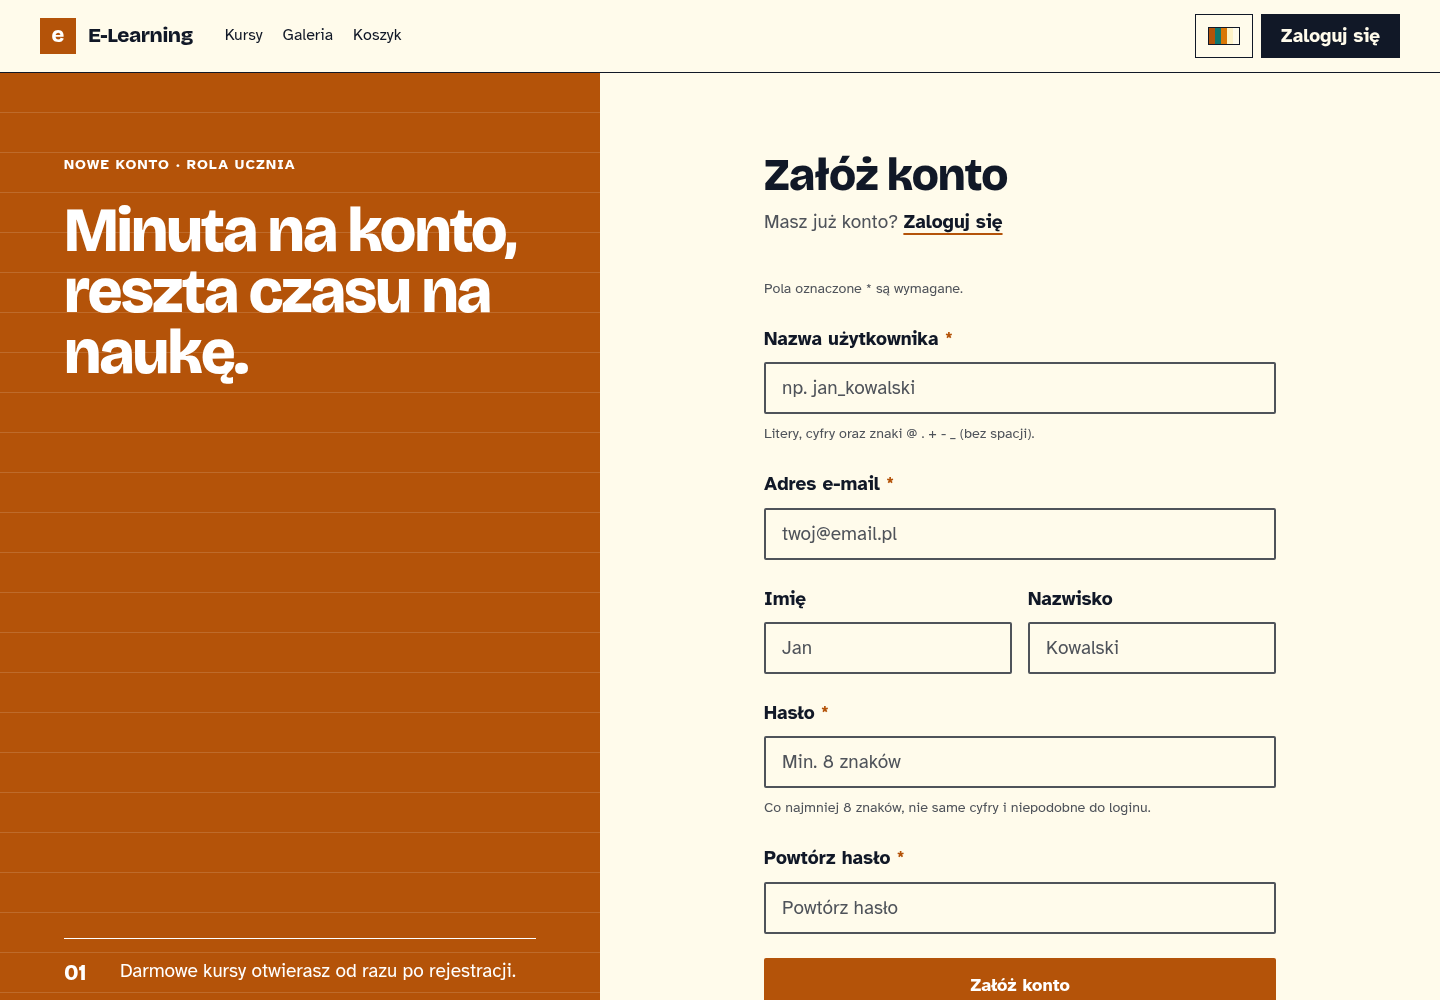
\includegraphics[width=0.94\linewidth,height=0.37\textheight,keepaspectratio]{img/register.png}}
\caption{Rejestracja}\label{fig:ui-register}
\end{figure}
Dostępność loginu i~e-maila jest sprawdzana podczas pisania; przy błędzie formularz zachowuje dane poza hasłami.


\begin{figure}[H]
\centering
\fcolorbox{rule}{white}{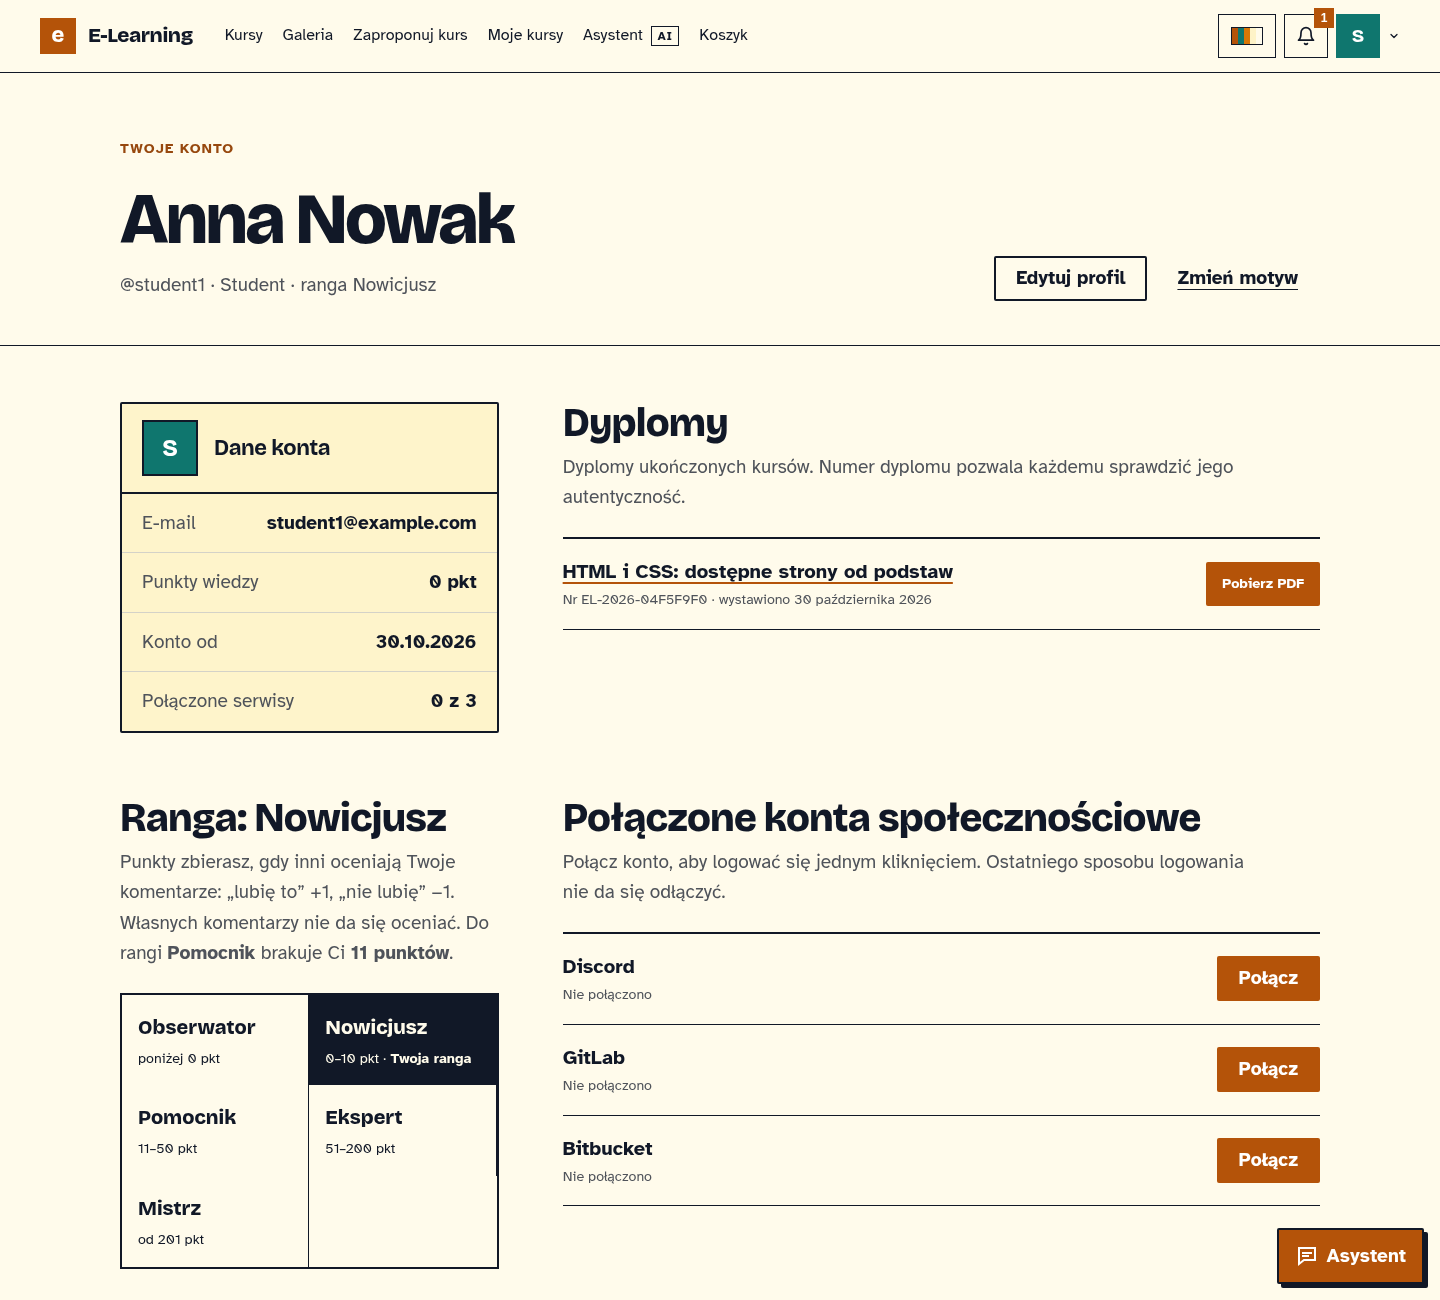
\includegraphics[width=0.94\linewidth,height=0.37\textheight,keepaspectratio]{img/profile.png}}
\caption{Profil ucznia}\label{fig:ui-profile}
\end{figure}
Dane konta, dyplomy do pobrania, ranga z~drabiną rang (ile punktów do następnej) i~połączone konta portali z~przyciskami łączenia/odłączania.


\begin{figure}[H]
\centering
\fcolorbox{rule}{white}{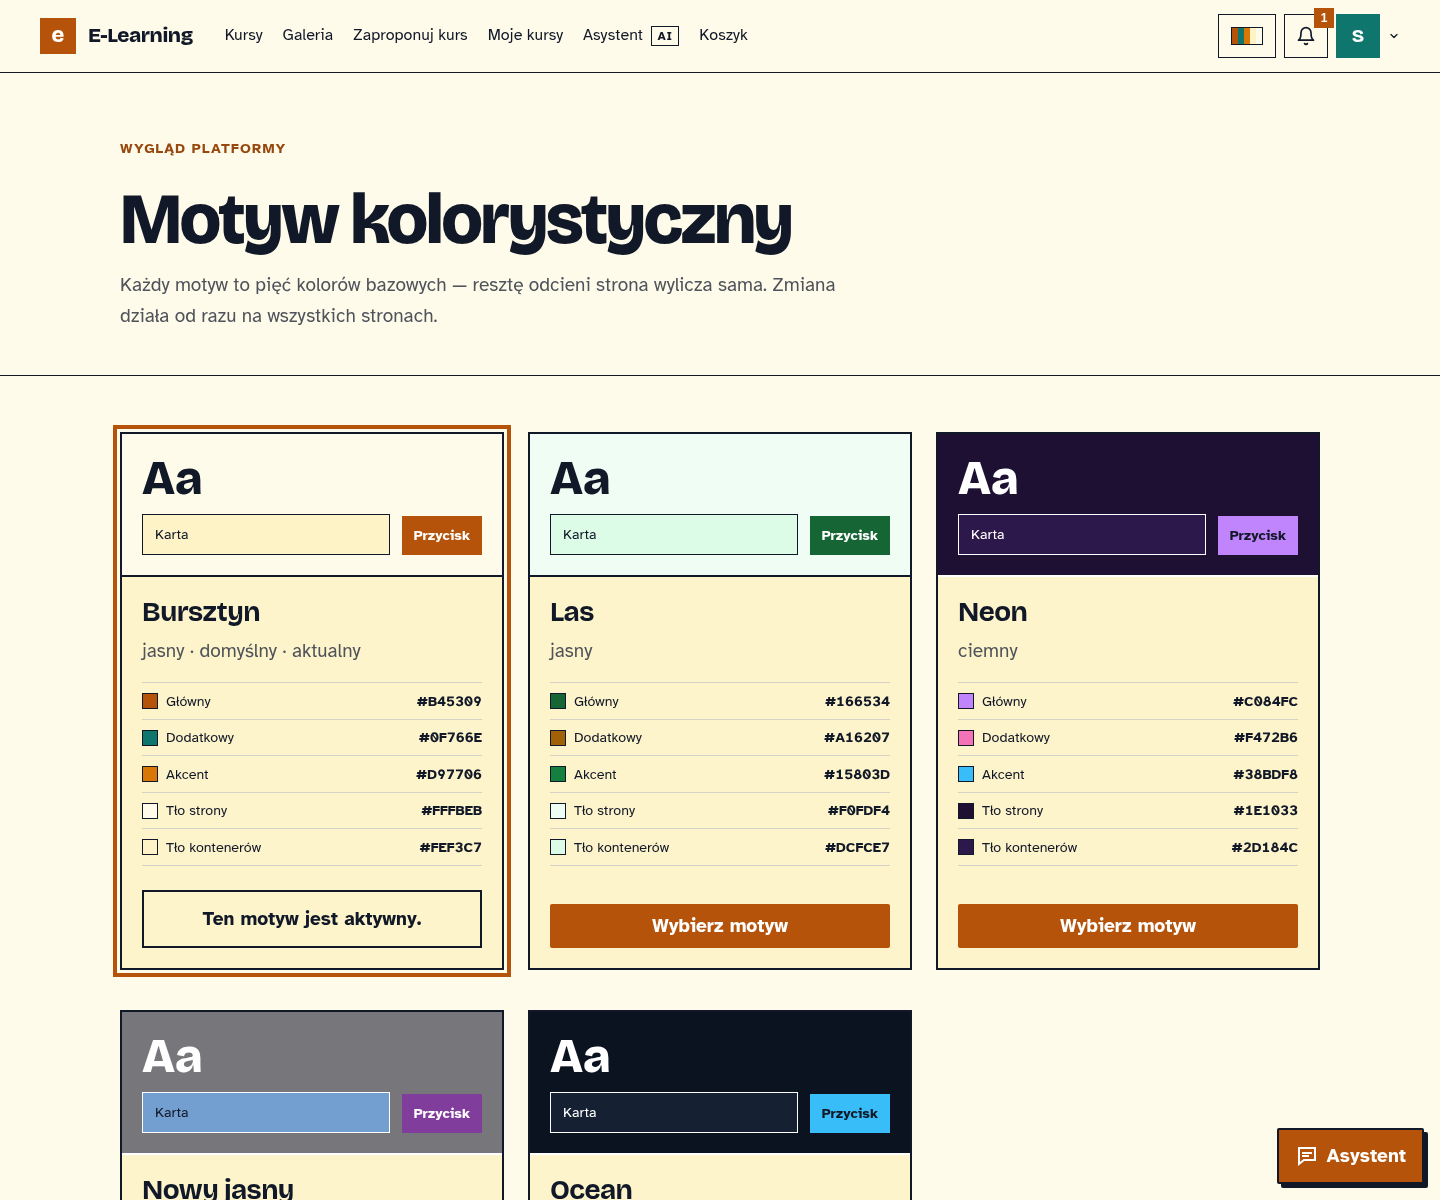
\includegraphics[width=0.94\linewidth,height=0.37\textheight,keepaspectratio]{img/themes.png}}
\caption{Wybór motywu}\label{fig:ui-themes}
\end{figure}
Każdy motyw jest pokazany na próbce interfejsu; wybór zapisuje się w~profilu.


\section{Katalog i~kurs}

\begin{figure}[H]
\centering
\fcolorbox{rule}{white}{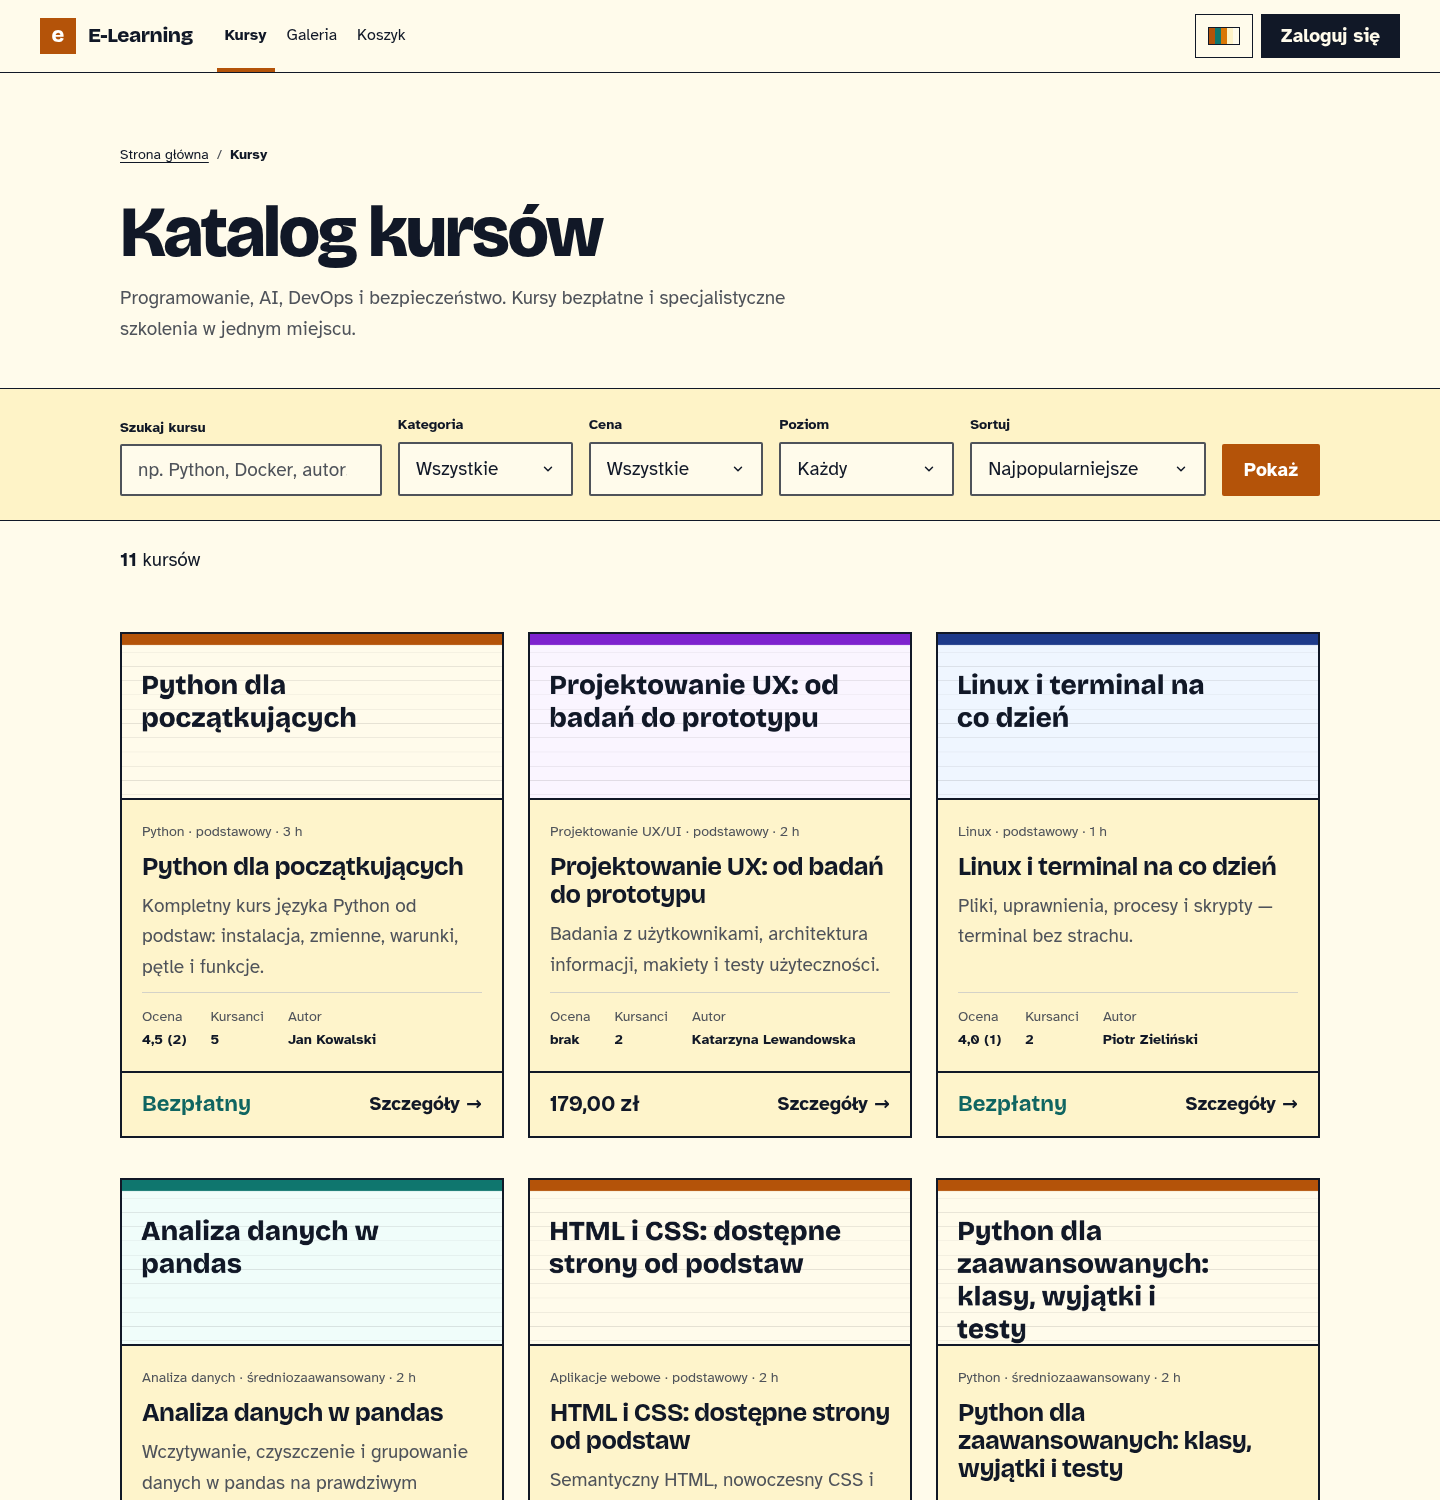
\includegraphics[width=0.94\linewidth,height=0.37\textheight,keepaspectratio]{img/catalog.png}}
\caption{Katalog kursów}\label{fig:ui-catalog}
\end{figure}
Wyszukiwarka i~filtry (kategoria, poziom, cena, sortowanie) w~jednym pasku, siatka kart w~trzech kolumnach, paginacja.


\begin{figure}[H]
\centering
\fcolorbox{rule}{white}{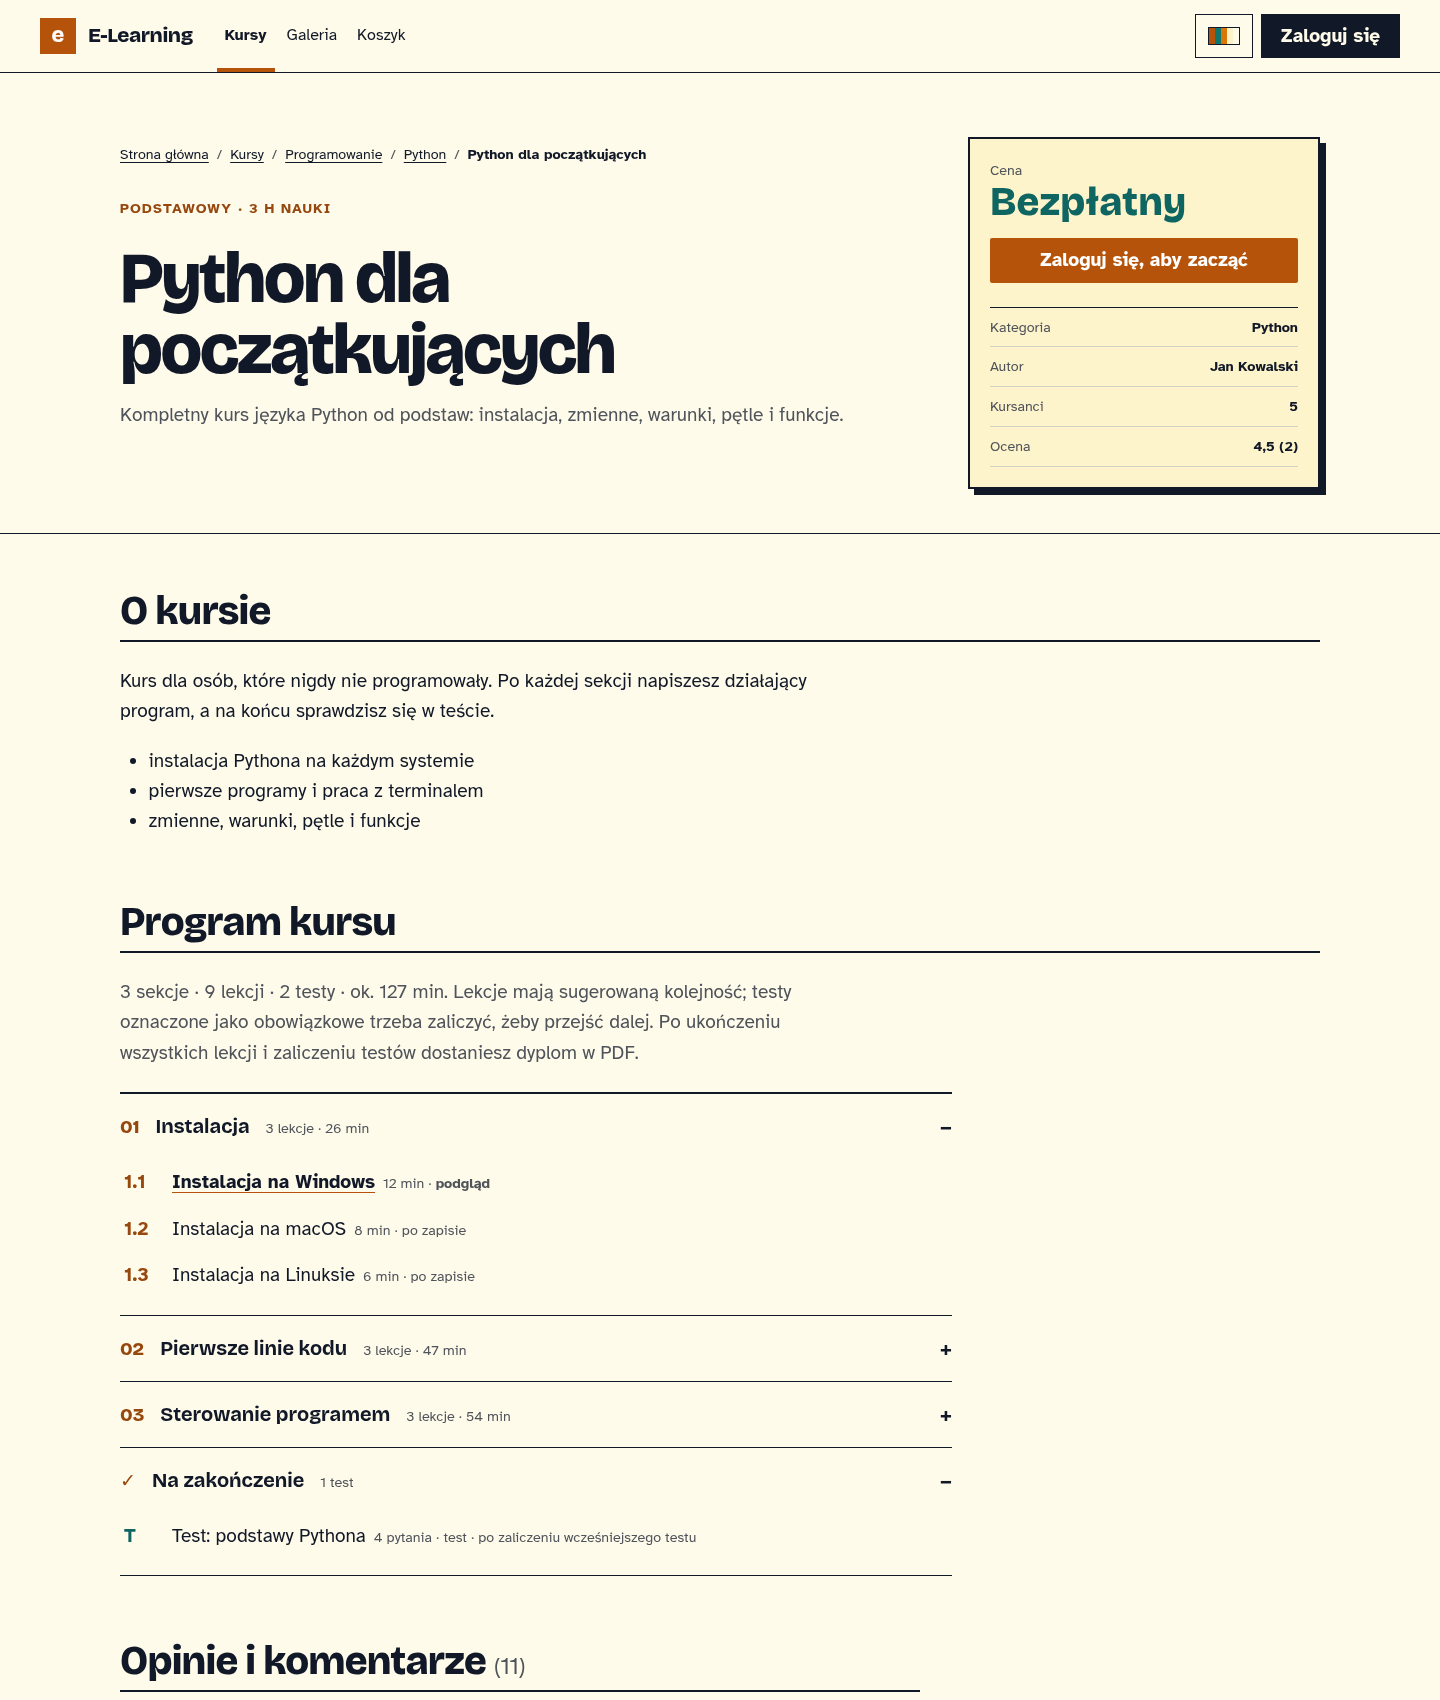
\includegraphics[width=0.94\linewidth,height=0.37\textheight,keepaspectratio]{img/course.png}}
\caption{Strona kursu}\label{fig:ui-course}
\end{figure}
Okruszki, opis ,,O kursie'', program z~czasem trwania, panel zakupu z~ceną lub przyciskiem zapisu oraz komentarze w~wątkach.


\section{Nauka}

\begin{figure}[H]
\centering
\fcolorbox{rule}{white}{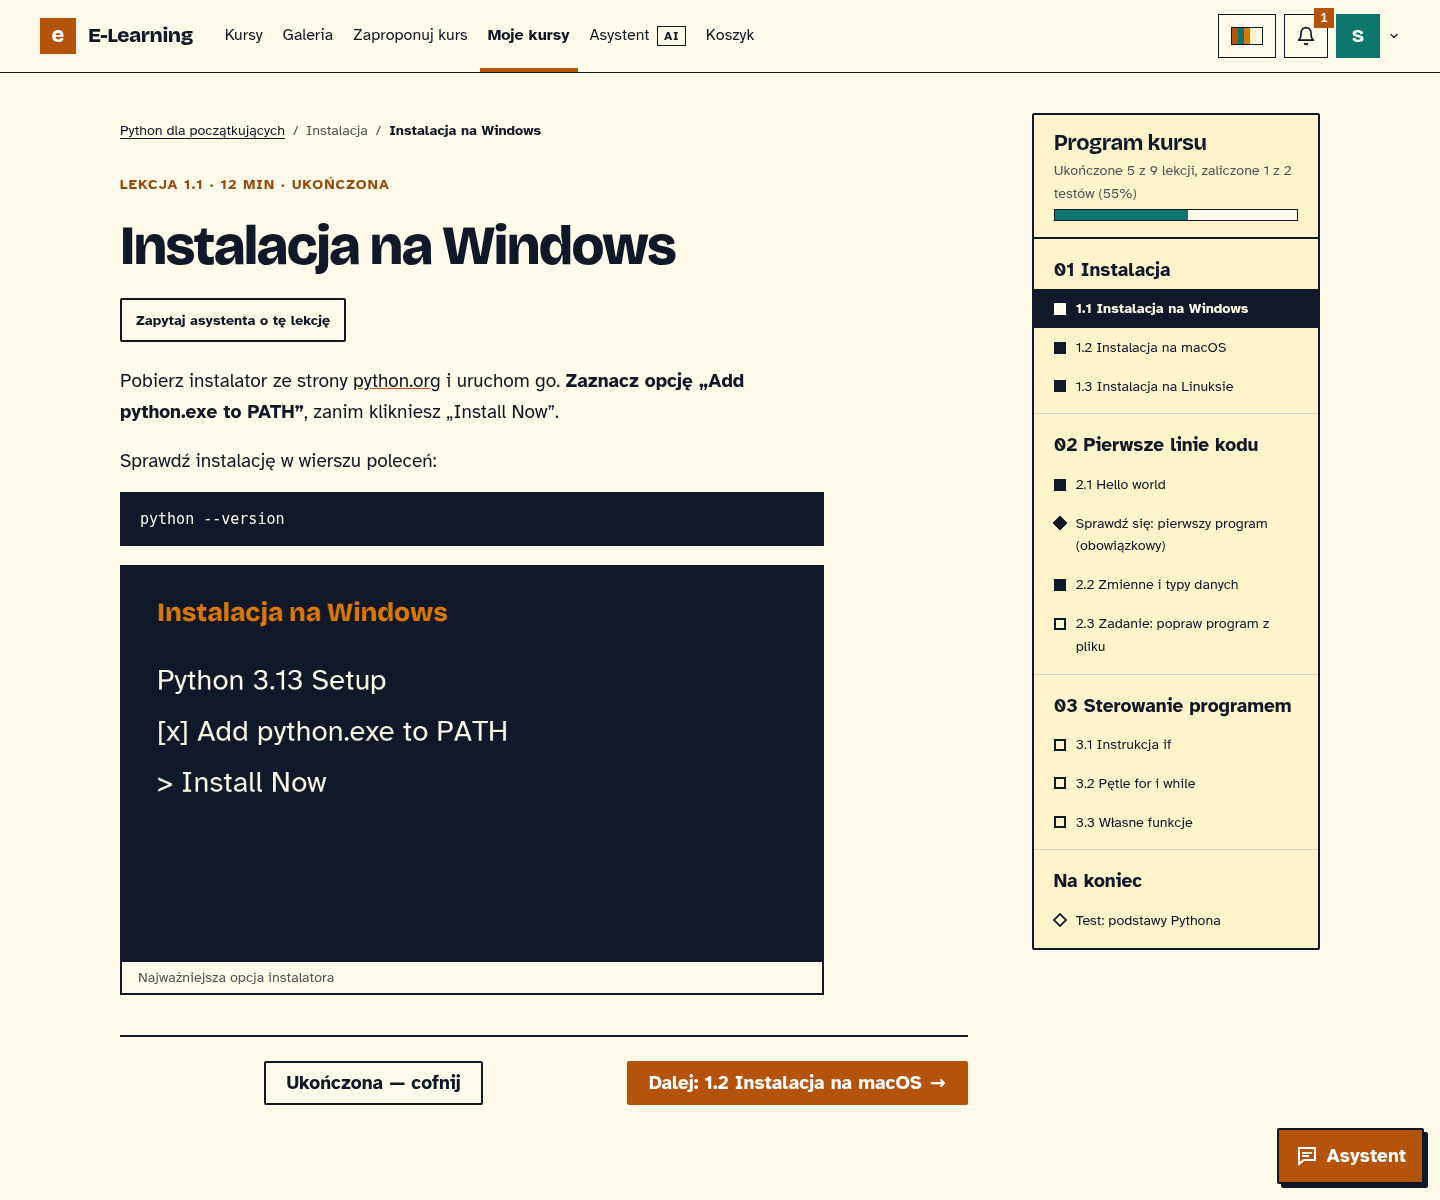
\includegraphics[width=0.94\linewidth,height=0.37\textheight,keepaspectratio]{img/lesson.png}}
\caption{Lekcja z~programem kursu}\label{fig:ui-lesson}
\end{figure}
Po lewej treść lekcji (kod, zdjęcie z~podpisem), po prawej program z~postępem i~oznaczeniami: ukończona (pełny kwadrat), test (romb), test obowiązkowy. Przycisk ,,Zapytaj asystenta o~tę lekcję'' otwiera czat z~kontekstem.


\begin{figure}[H]
\centering
\fcolorbox{rule}{white}{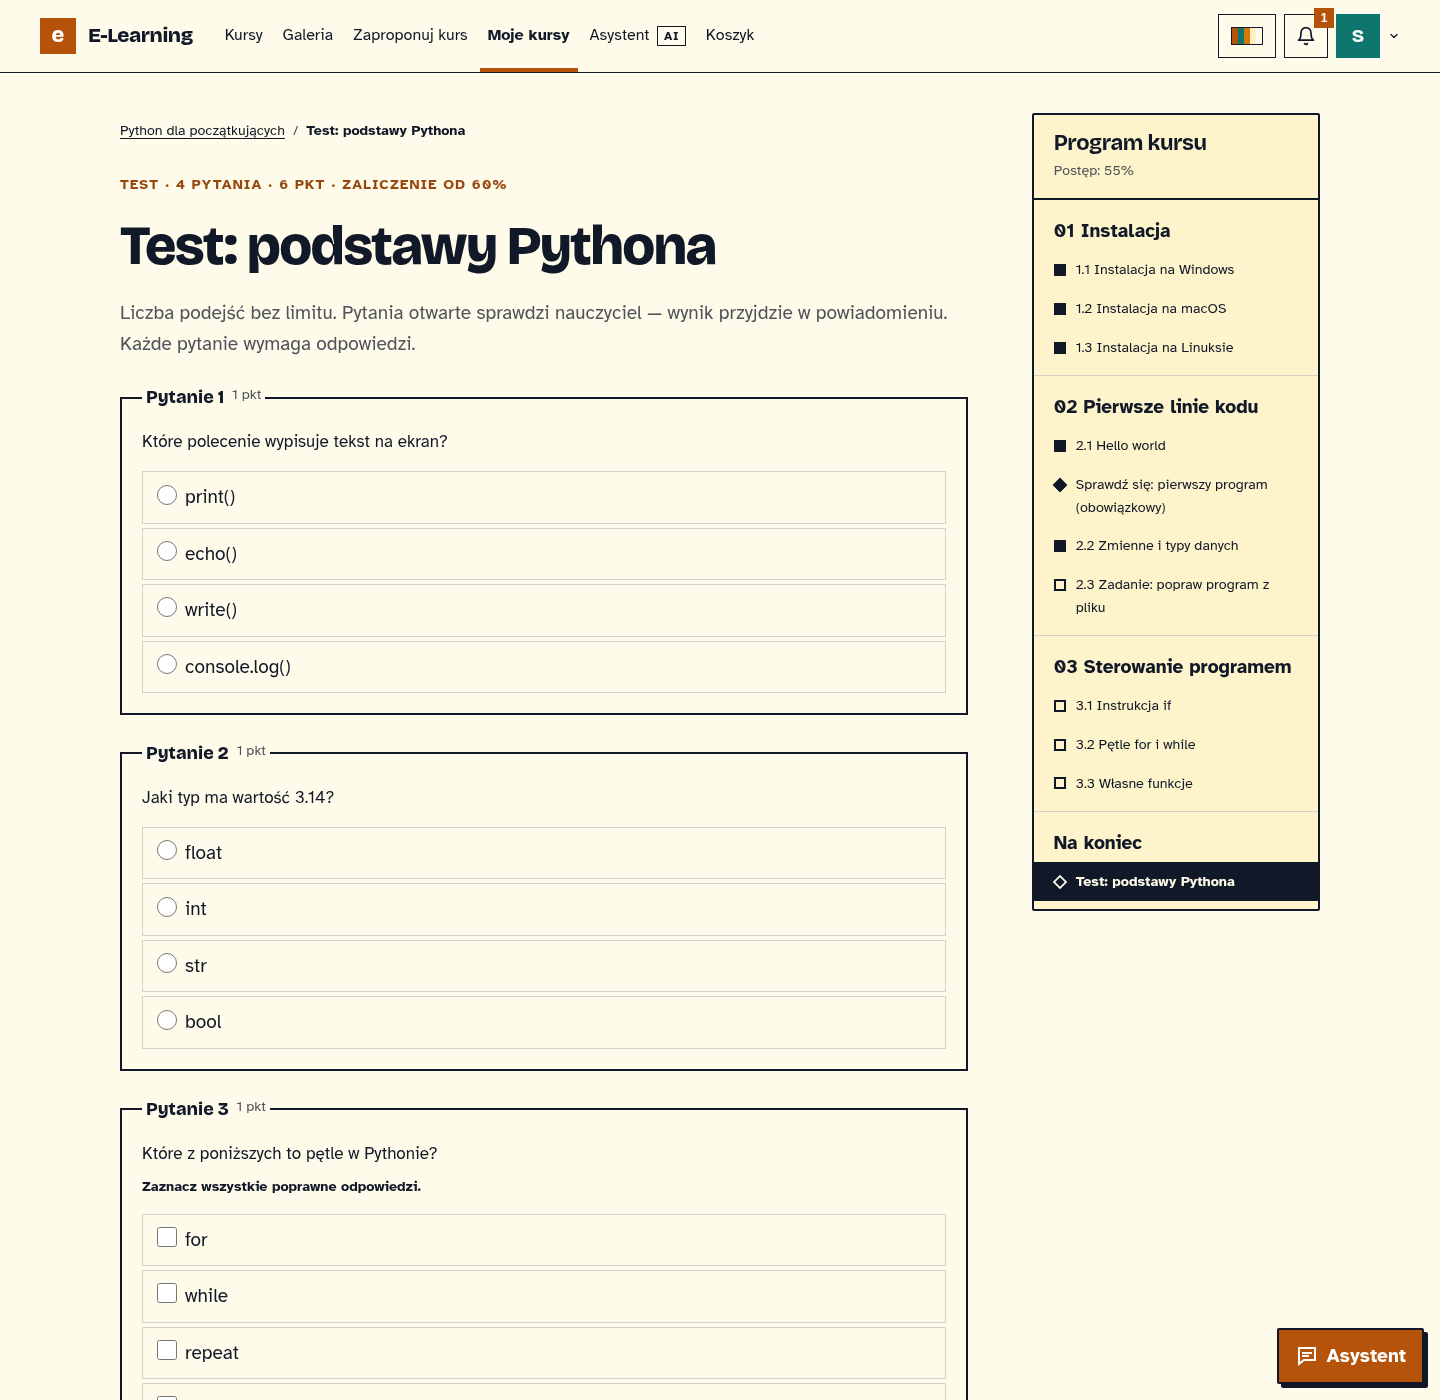
\includegraphics[width=0.94\linewidth,height=0.37\textheight,keepaspectratio]{img/quiz.png}}
\caption{Rozwiązywanie testu}\label{fig:ui-quiz}
\end{figure}
Każde pytanie to \code{fieldset} z~\code{legend} (numer i~punkty); odpowiedzi jednokrotnego wyboru jako pola radio, wielokrotnego -- pola wyboru z~instrukcją ,,Zaznacz wszystkie poprawne odpowiedzi''.


\begin{figure}[H]
\centering
\fcolorbox{rule}{white}{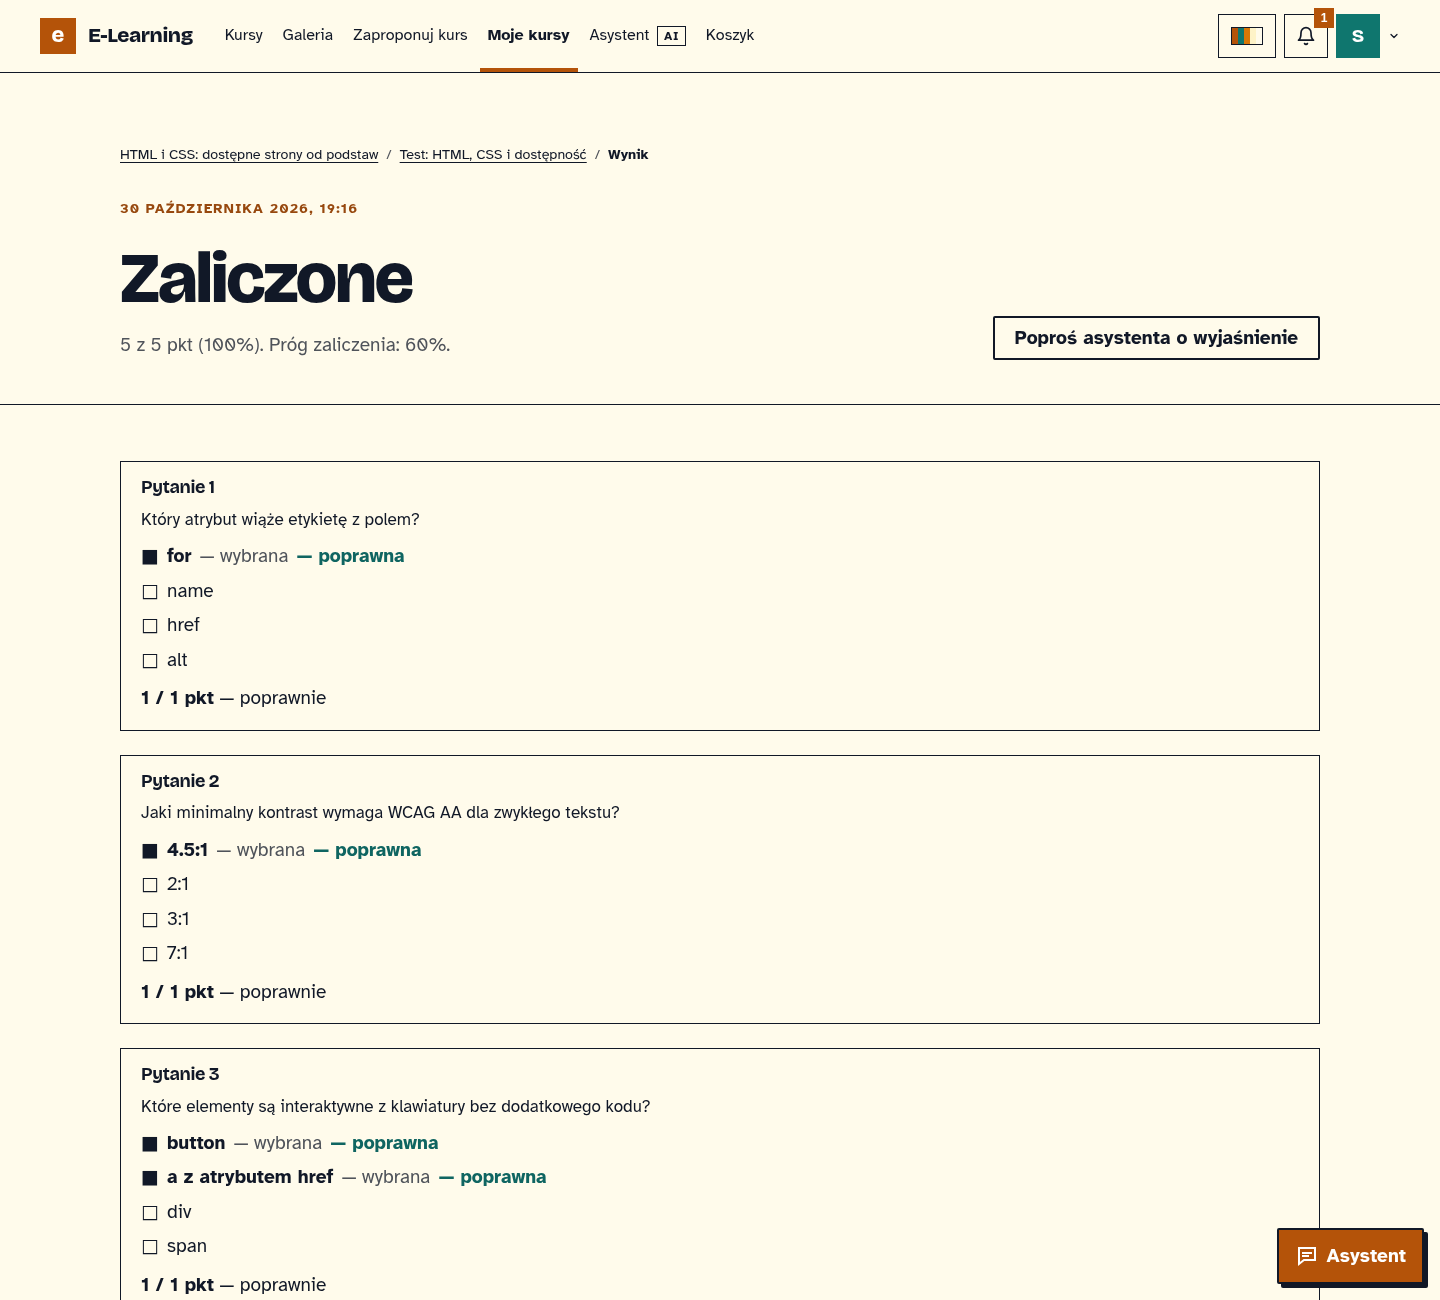
\includegraphics[width=0.94\linewidth,height=0.37\textheight,keepaspectratio]{img/attempt.png}}
\caption{Wynik testu}\label{fig:ui-attempt}
\end{figure}
Wynik procentowy, punkty za każde pytanie, poprawne odpowiedzi (po zaliczeniu) i~przycisk ,,Poproś asystenta o~wyjaśnienie''.


\begin{figure}[H]
\centering
\fcolorbox{rule}{white}{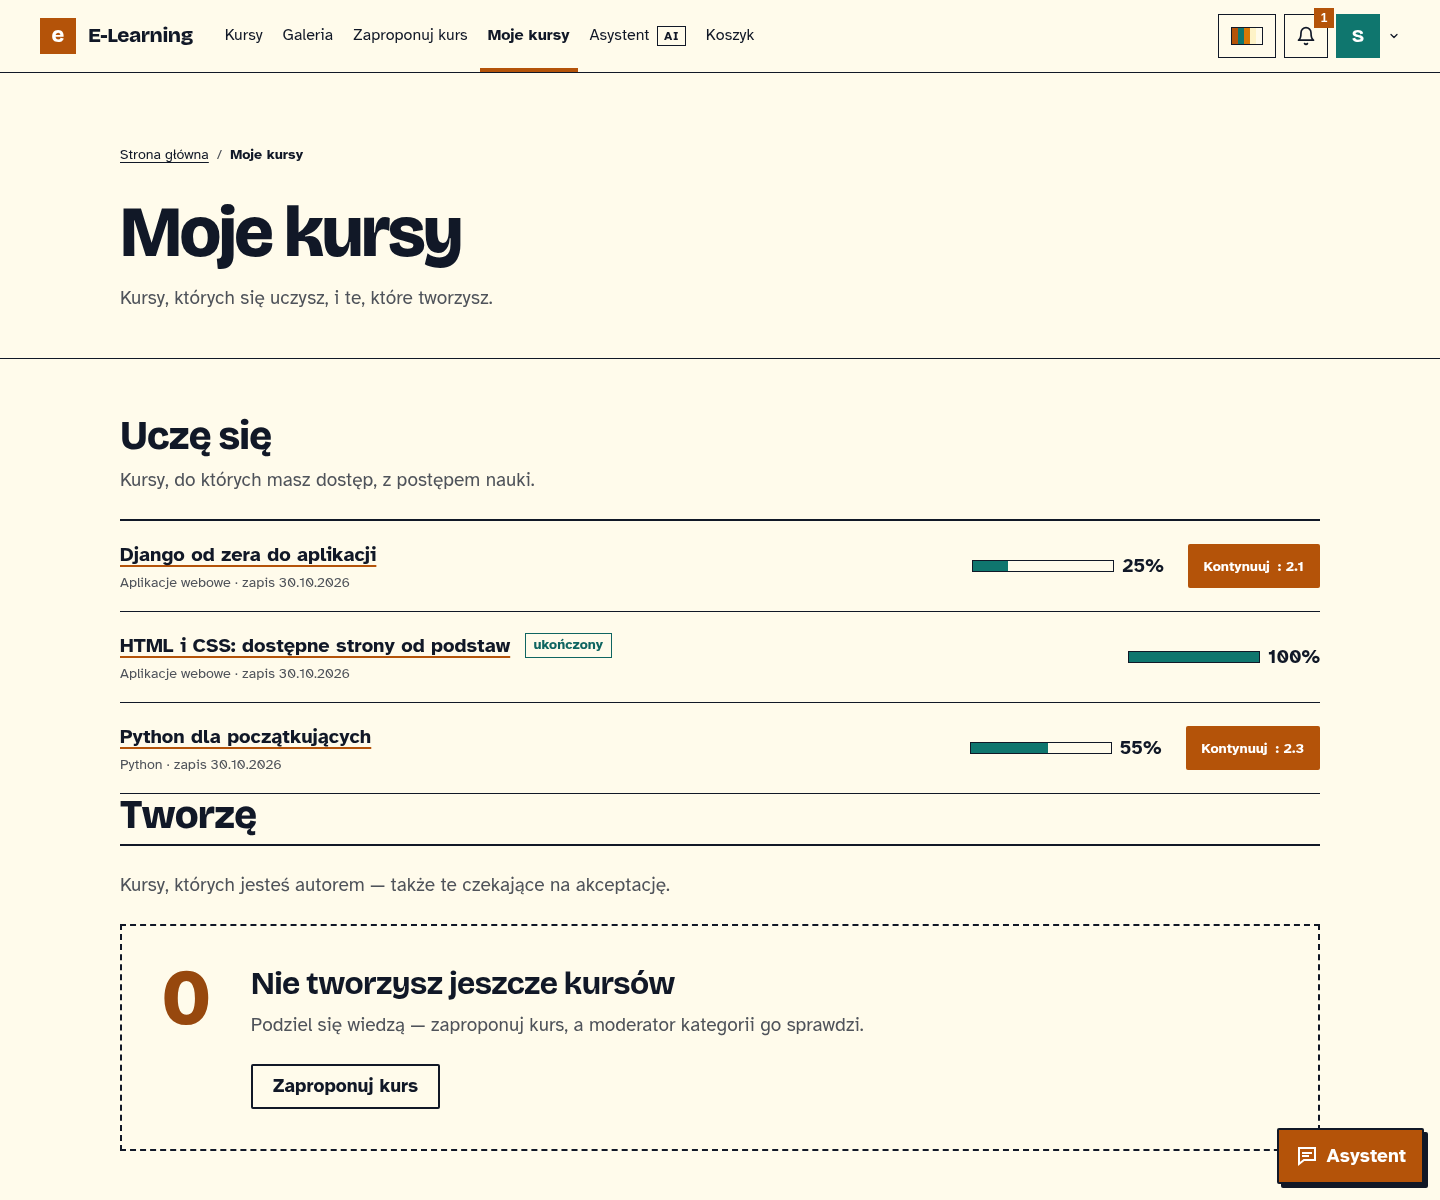
\includegraphics[width=0.94\linewidth,height=0.37\textheight,keepaspectratio]{img/mycourses.png}}
\caption{Moje kursy}\label{fig:ui-mycourses}
\end{figure}
Zakładka ,,Uczę się'' z~paskami postępu i~,,Tworzę'' ze stanem zgłoszeń; pusta sekcja pokazuje stan pusty z~zachętą.


\section{Asystent AI}

\begin{figure}[H]
\centering
\fcolorbox{rule}{white}{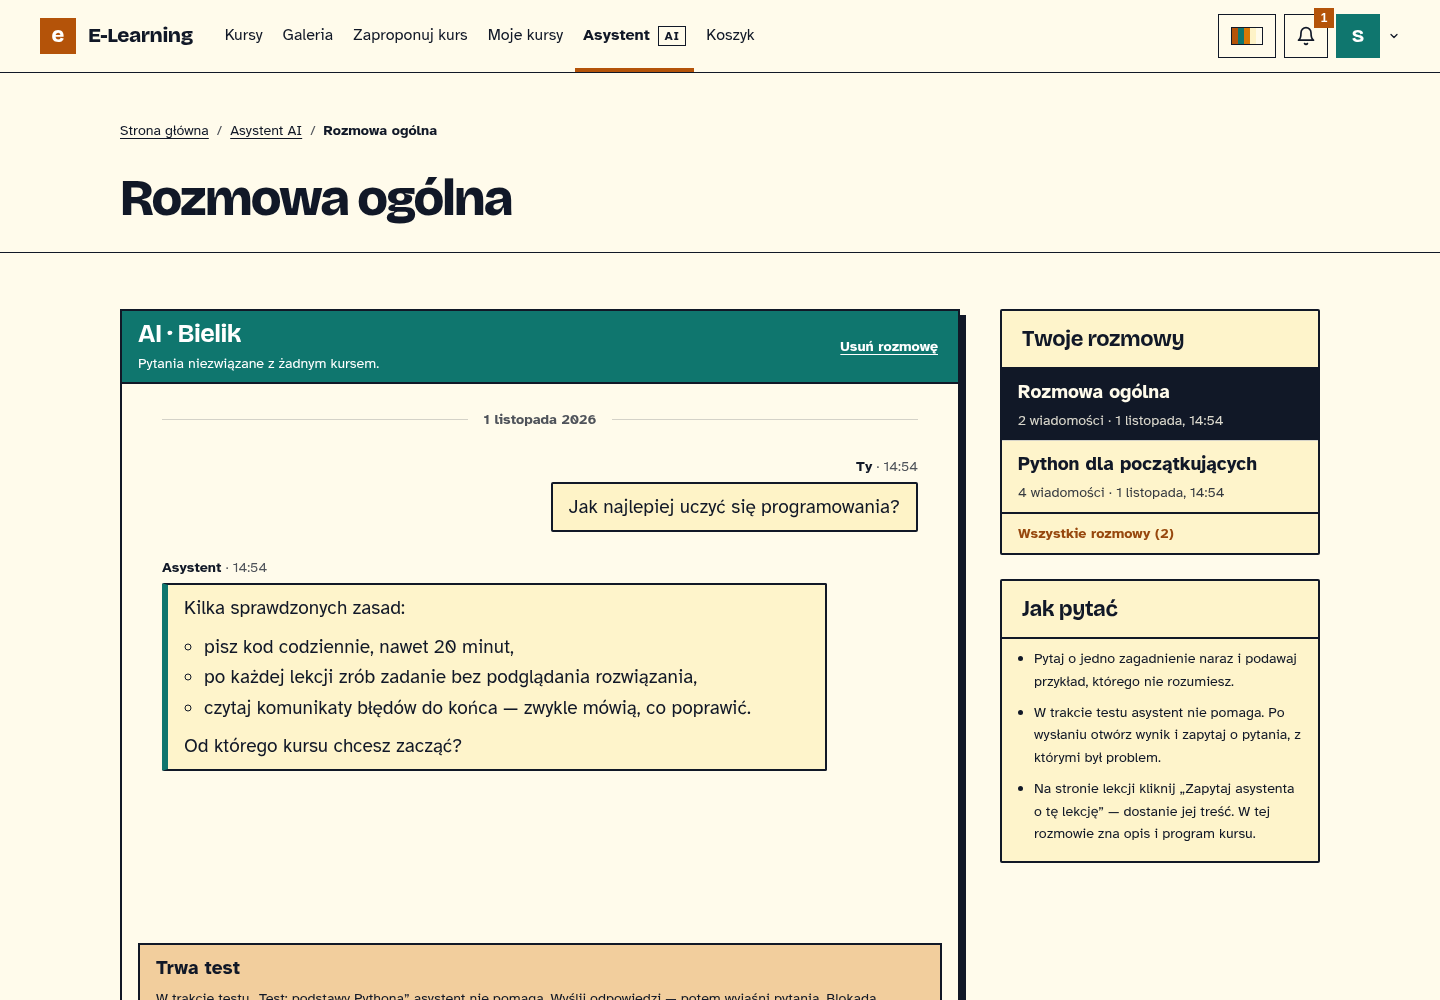
\includegraphics[width=0.94\linewidth,height=0.37\textheight,keepaspectratio]{img/chat.png}}
\caption{Strona rozmowy z~asystentem}\label{fig:ui-chat}
\end{figure}
Ramka czatu z~historią i~boczną listą rozmów (ogólna i~po jednej na kurs). Odpowiedzi są formatowane (listy, pogrubienia, kod).


\section{Sklep}

\begin{figure}[H]
\centering
\fcolorbox{rule}{white}{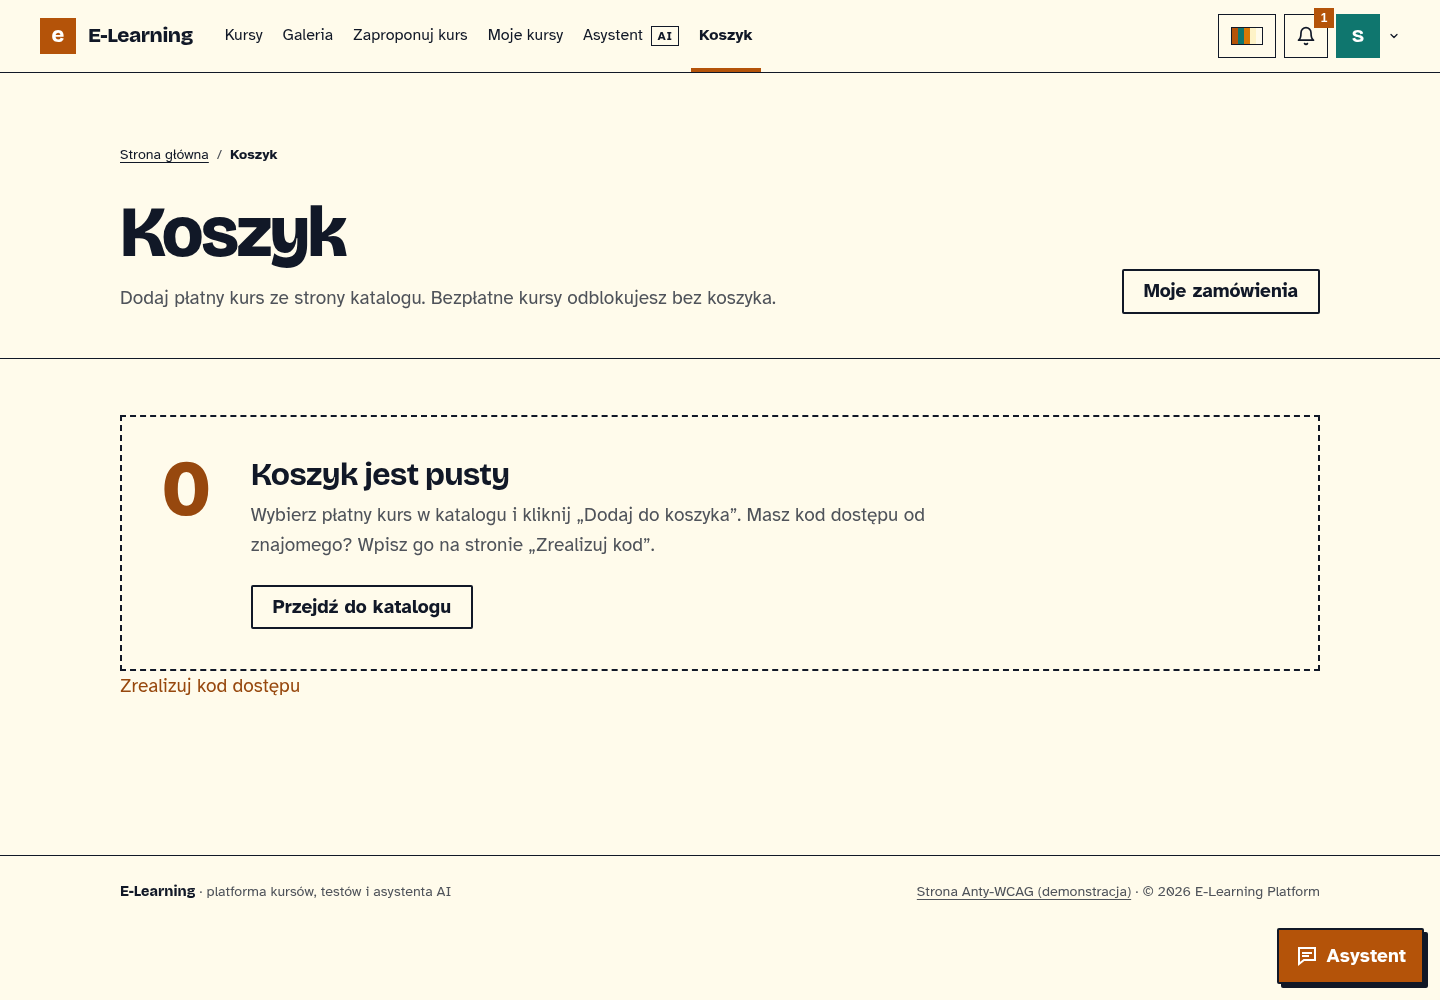
\includegraphics[width=0.94\linewidth,height=0.37\textheight,keepaspectratio]{img/cart.png}}
\caption{Koszyk -- stan pusty}\label{fig:ui-cart}
\end{figure}
Pusta lista nigdy nie jest pustą tabelą: komponent stanu pustego wyjaśnia sytuację i~proponuje następną akcję.


\begin{figure}[H]
\centering
\fcolorbox{rule}{white}{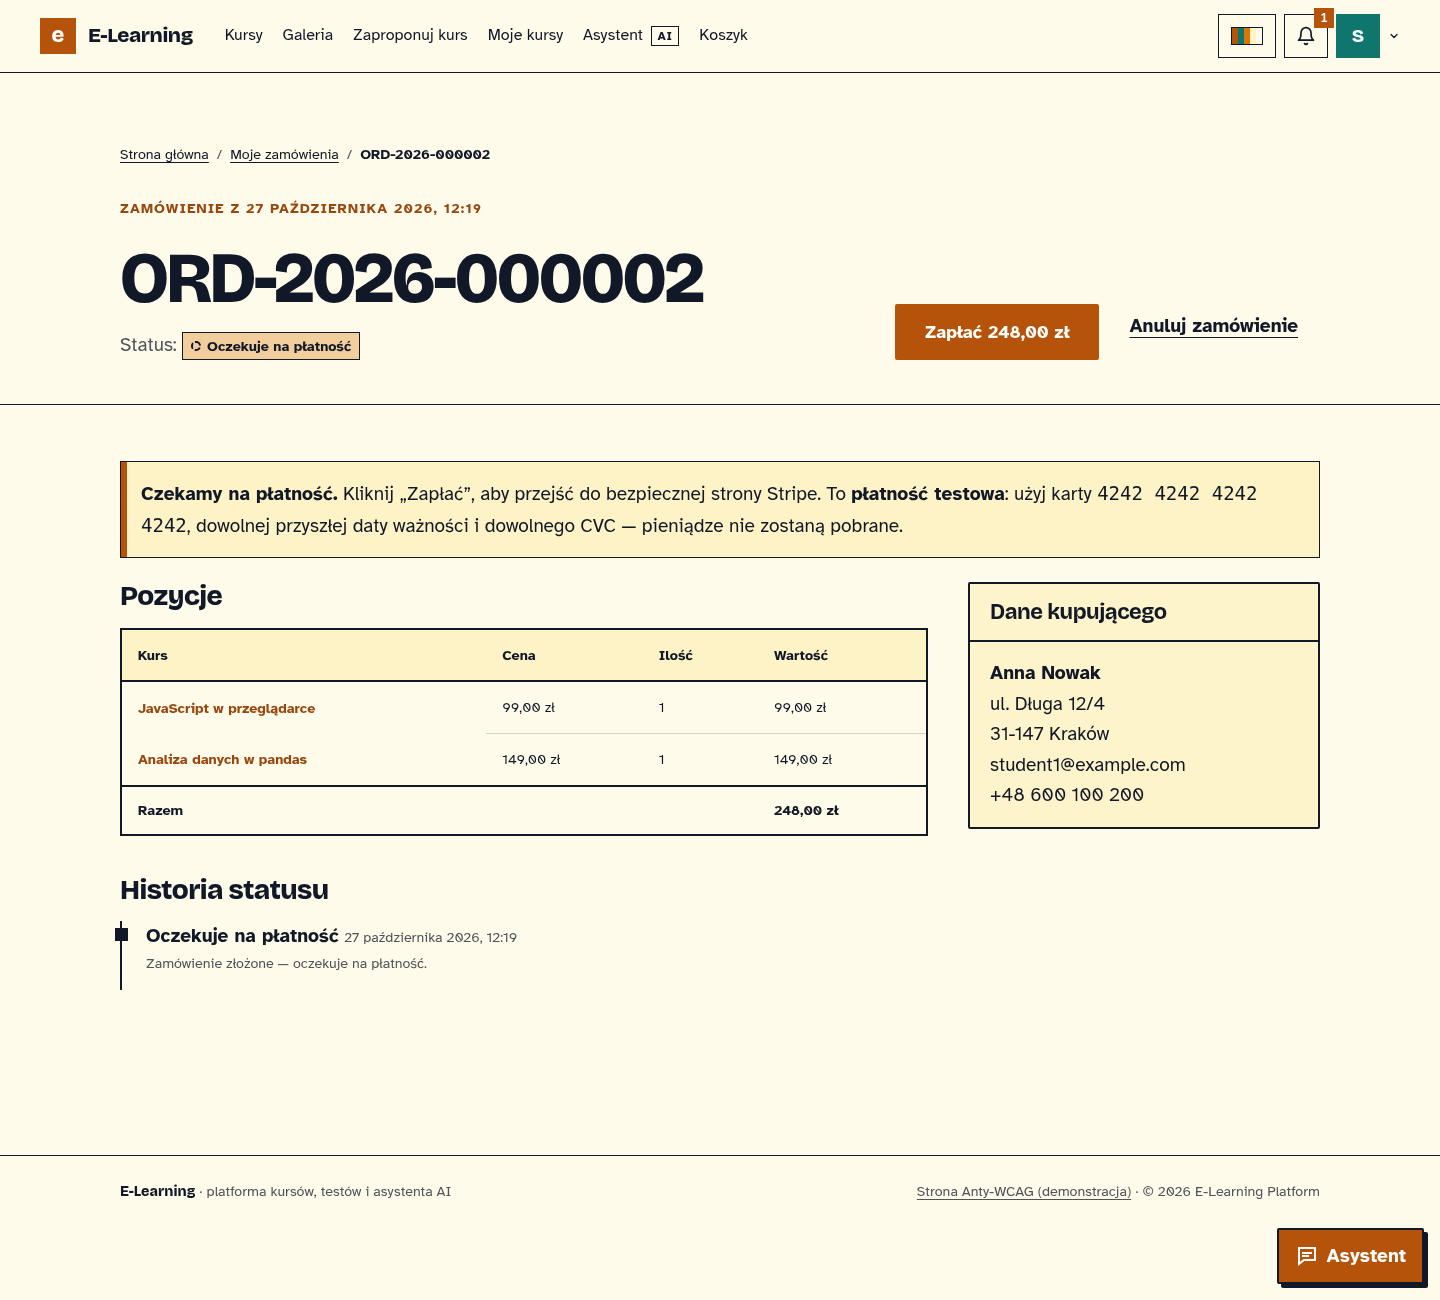
\includegraphics[width=0.94\linewidth,height=0.37\textheight,keepaspectratio]{img/order.png}}
\caption{Szczegóły zamówienia}\label{fig:ui-order}
\end{figure}
Numer, status, pozycje z~kodami dostępu, dane kupującego i~historia statusów; dla nieopłaconego zamówienia -- przycisk ,,Zapłać'' prowadzący do Stripe.


\section{Moderacja i~zarządzanie}

\begin{figure}[H]
\centering
\fcolorbox{rule}{white}{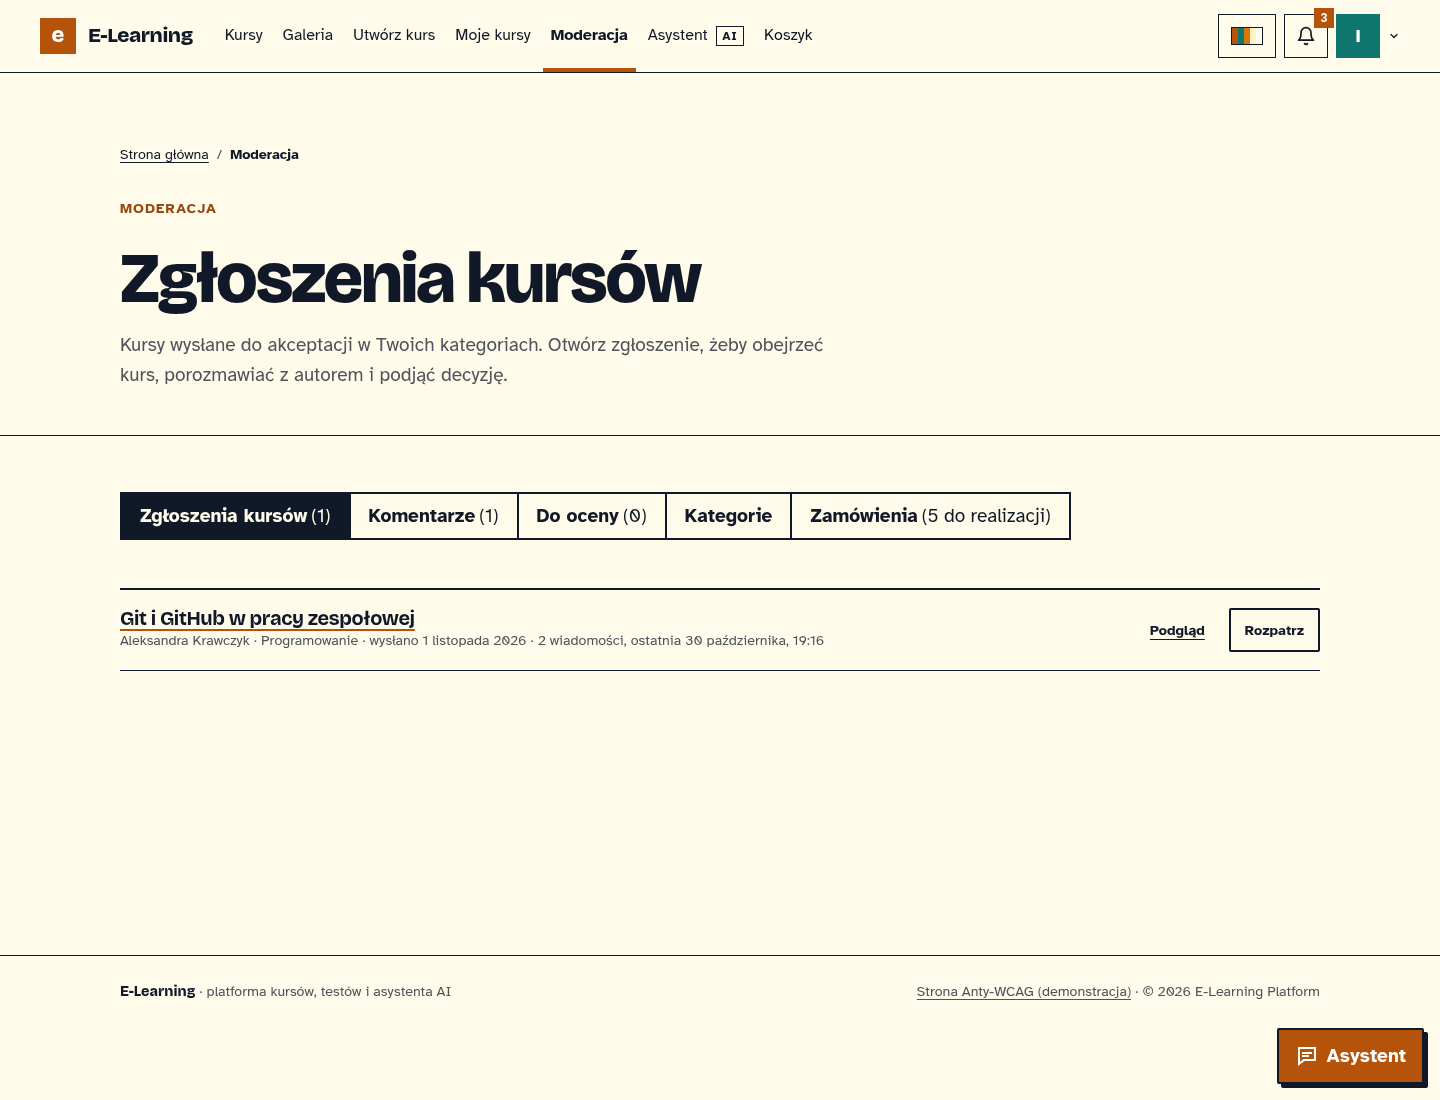
\includegraphics[width=0.94\linewidth,height=0.37\textheight,keepaspectratio]{img/moderation.png}}
\caption{Moderacja -- zgłoszenia kursów}\label{fig:ui-moderation}
\end{figure}
Zakładki: Zgłoszenia, Komentarze, Do oceny, Kategorie, Zamówienia -- z~licznikami oczekujących pozycji.


\begin{figure}[H]
\centering
\fcolorbox{rule}{white}{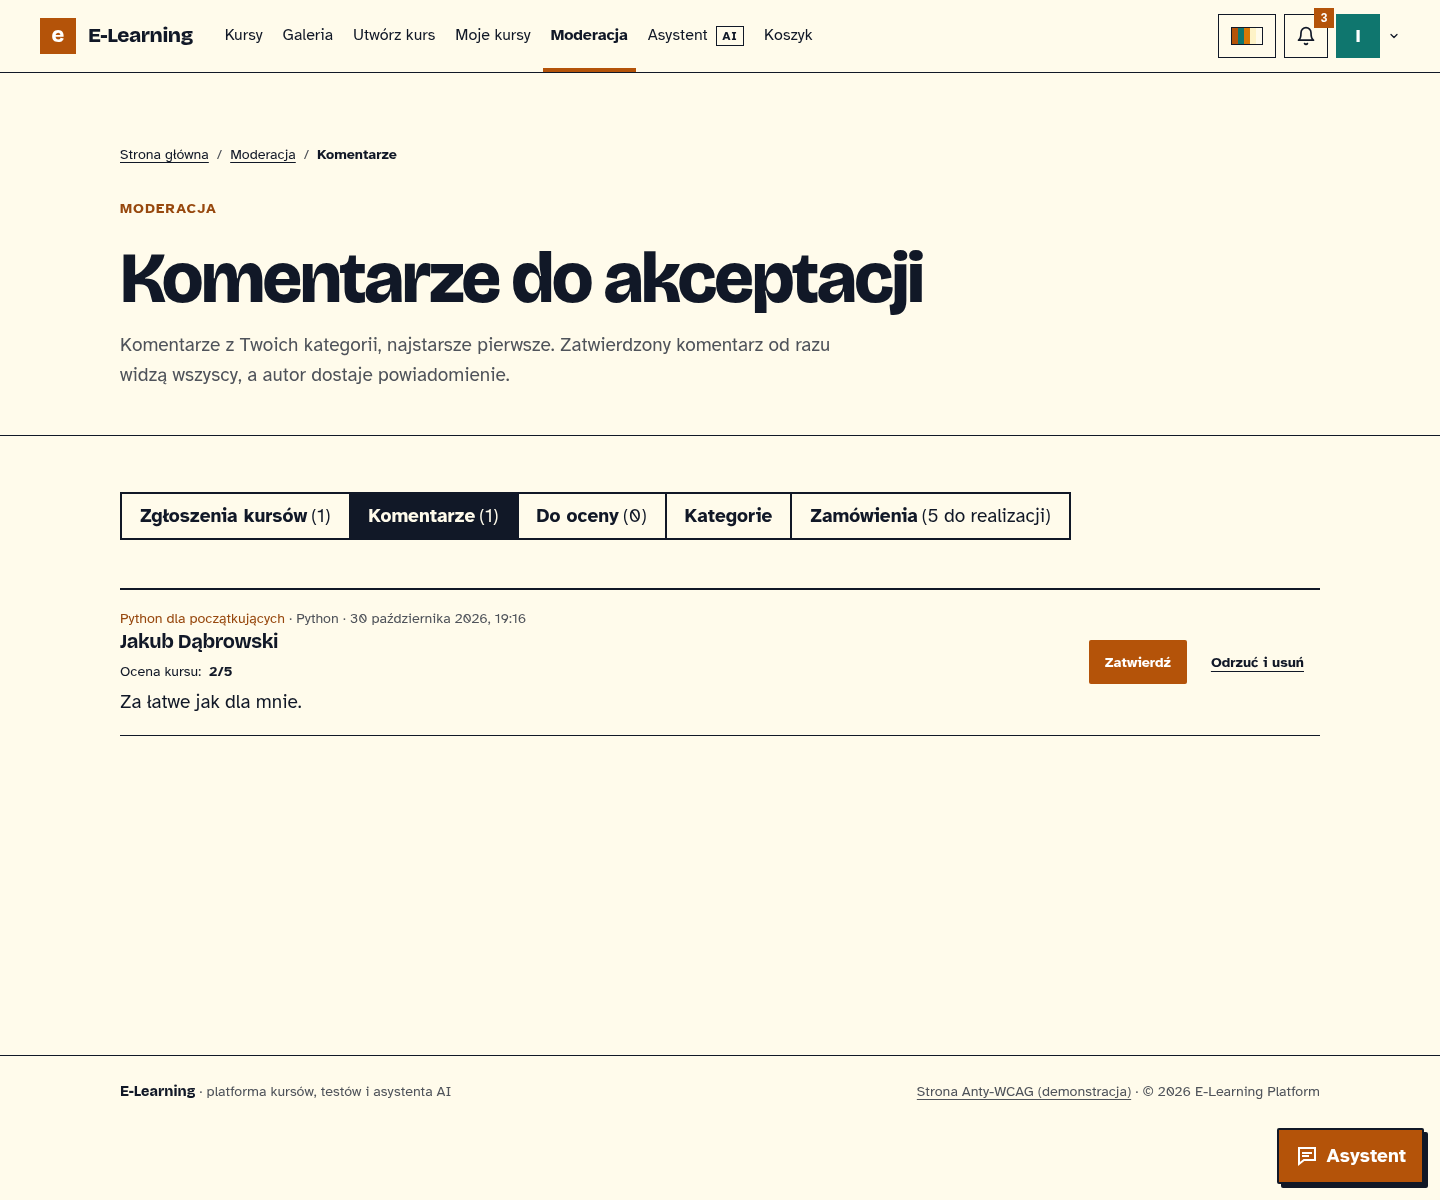
\includegraphics[width=0.94\linewidth,height=0.37\textheight,keepaspectratio]{img/mod_comments.png}}
\caption{Moderacja -- komentarze do akceptacji}\label{fig:ui-mod-comments}
\end{figure}
Akceptacja jednym kliknięciem, usunięcie z~dialogiem potwierdzenia.


\begin{figure}[H]
\centering
\fcolorbox{rule}{white}{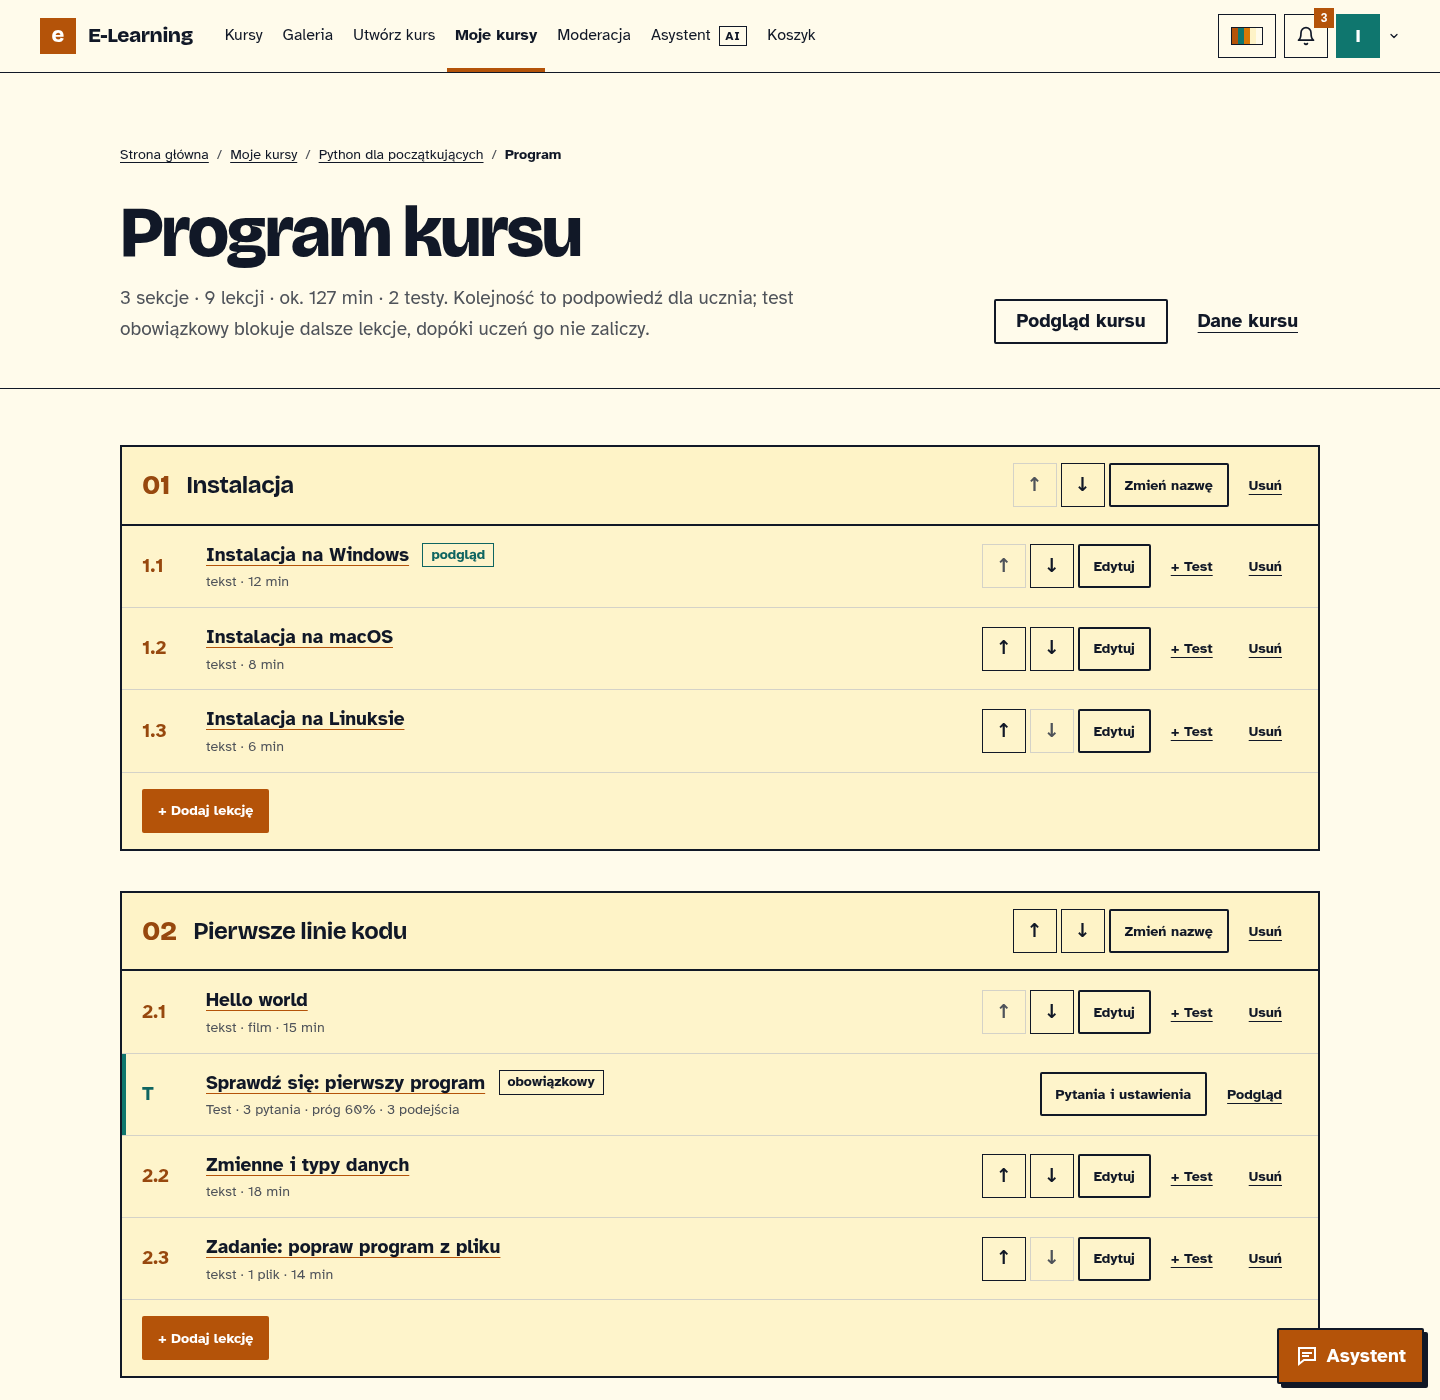
\includegraphics[width=0.94\linewidth,height=0.37\textheight,keepaspectratio]{img/curriculum.png}}
\caption{Kreator kursu -- krok 2: program}\label{fig:ui-curriculum}
\end{figure}
Sekcje i~lekcje z~przyciskami $\uparrow\downarrow$, edycją i~usuwaniem; testy wstawiane po lekcji lub na końcu.


\begin{figure}[H]
\centering
\fcolorbox{rule}{white}{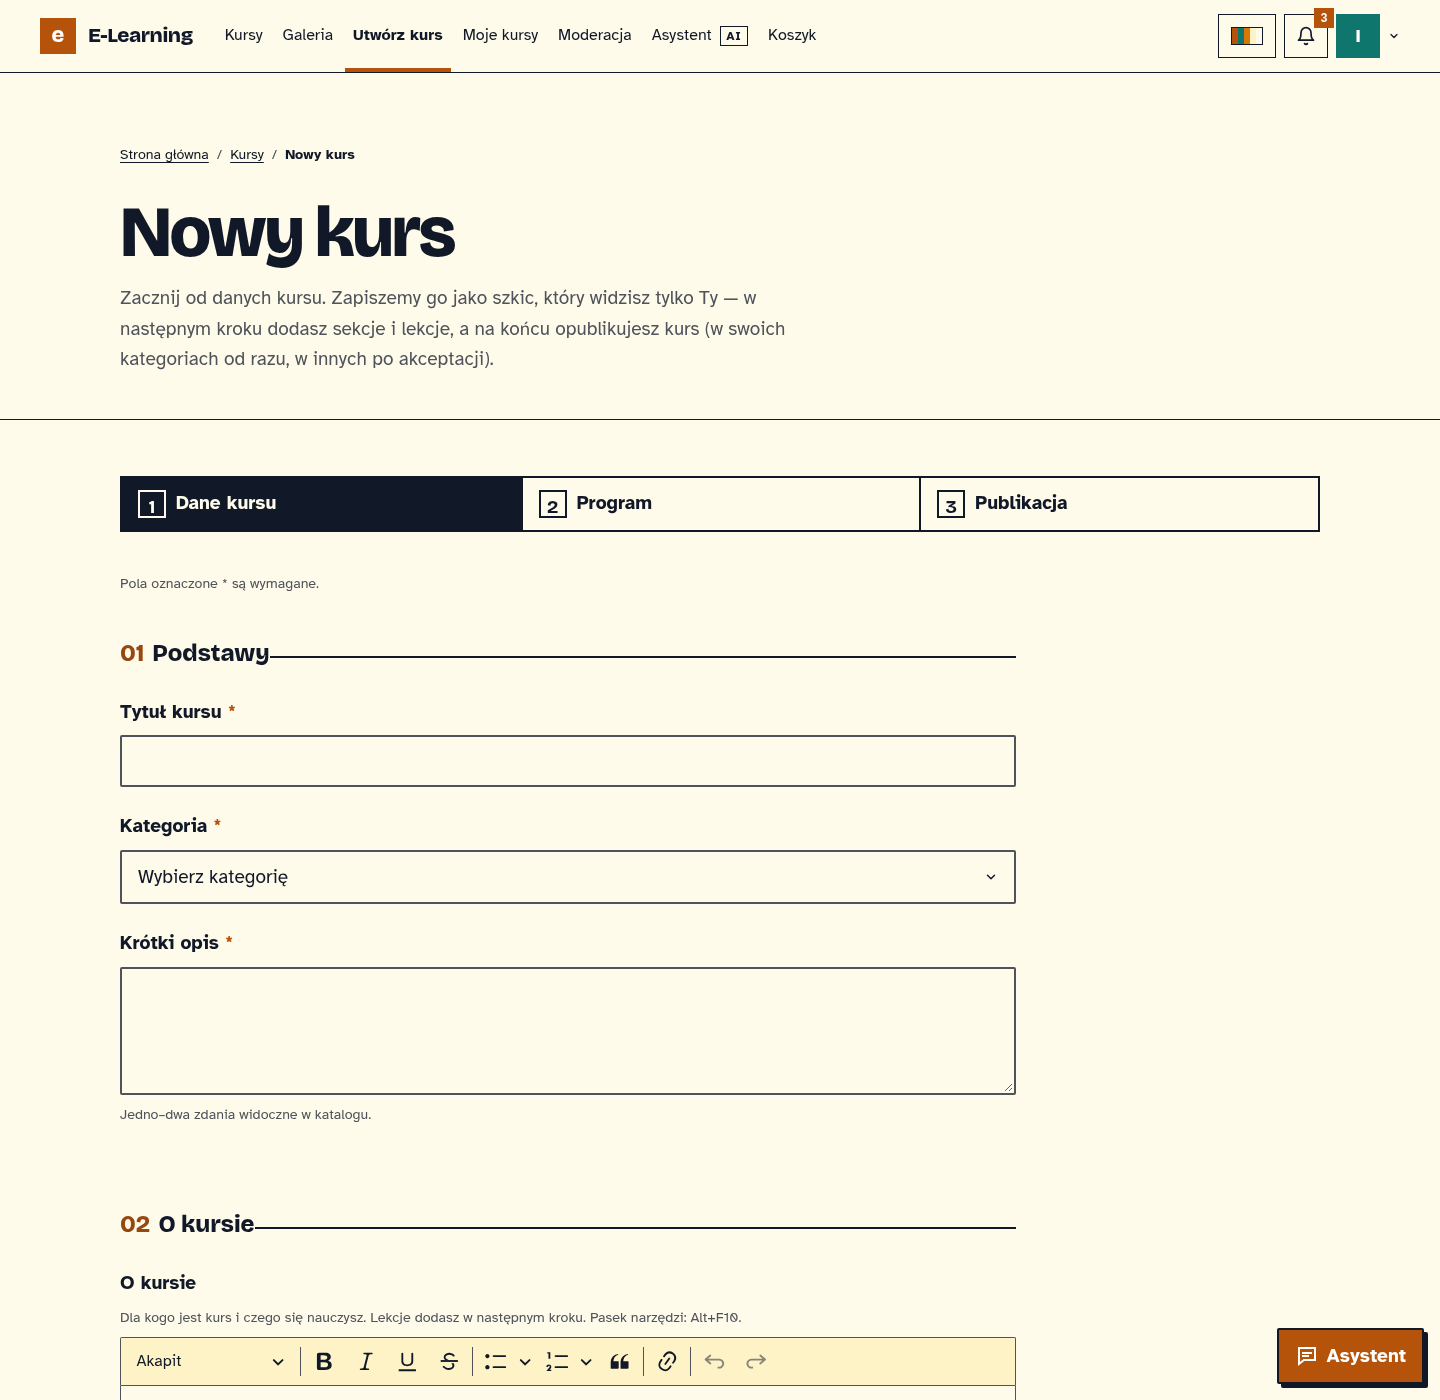
\includegraphics[width=0.94\linewidth,height=0.37\textheight,keepaspectratio]{img/course_create.png}}
\caption{Kreator kursu -- krok 1: dane}\label{fig:ui-course-create}
\end{figure}
Pasek kroków (Dane kursu -- Program -- Publikacja), pola z~etykietami, opis w~CKEditorze.


\begin{figure}[H]
\centering
\fcolorbox{rule}{white}{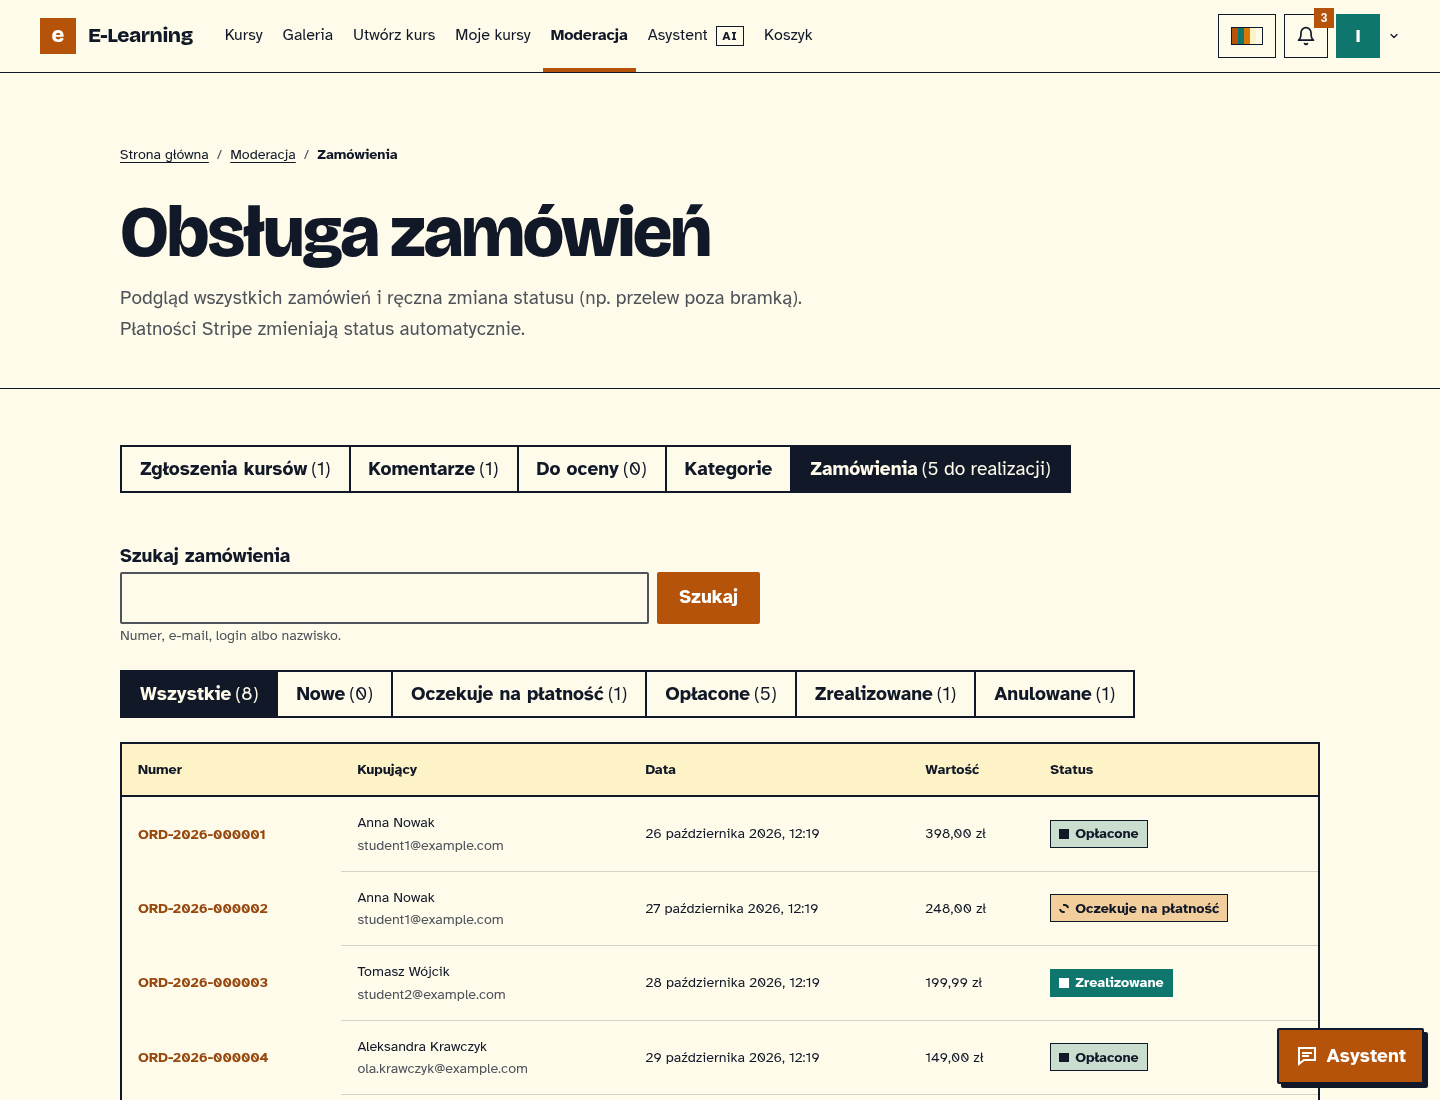
\includegraphics[width=0.94\linewidth,height=0.37\textheight,keepaspectratio]{img/orders_manage.png}}
\caption{Obsługa zamówień}\label{fig:ui-orders-manage}
\end{figure}
Filtr statusu jako przełącznik segmentowy, wyszukiwarka i~tabela z~paginacją.


\begin{figure}[H]
\centering
\fcolorbox{rule}{white}{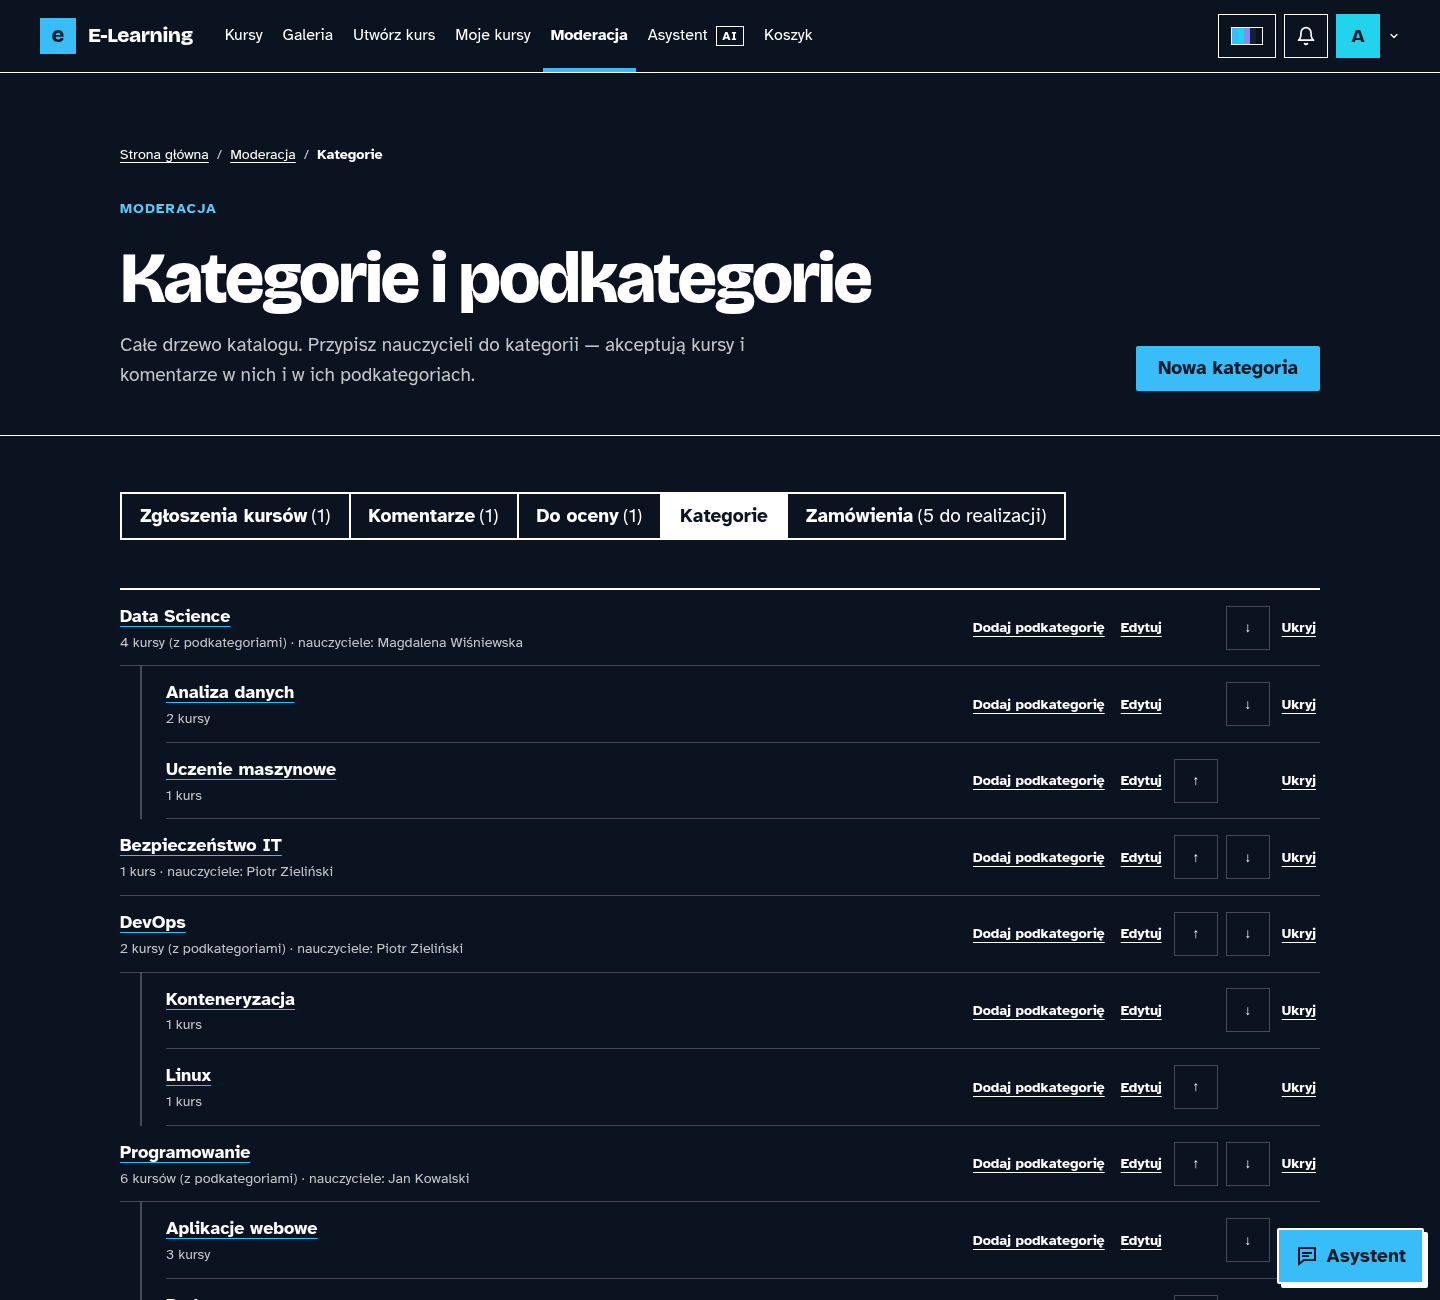
\includegraphics[width=0.94\linewidth,height=0.37\textheight,keepaspectratio]{img/categories.png}}
\caption{Zarządzanie kategoriami (administrator, motyw ciemny ,,Ocean'')}\label{fig:ui-categories}
\end{figure}
Drzewo z~liczbą kursów, dodawanie podkategorii, zmiana kolejności, ukrywanie i~przydział nauczycieli.


\begin{figure}[H]
\centering
\fcolorbox{rule}{white}{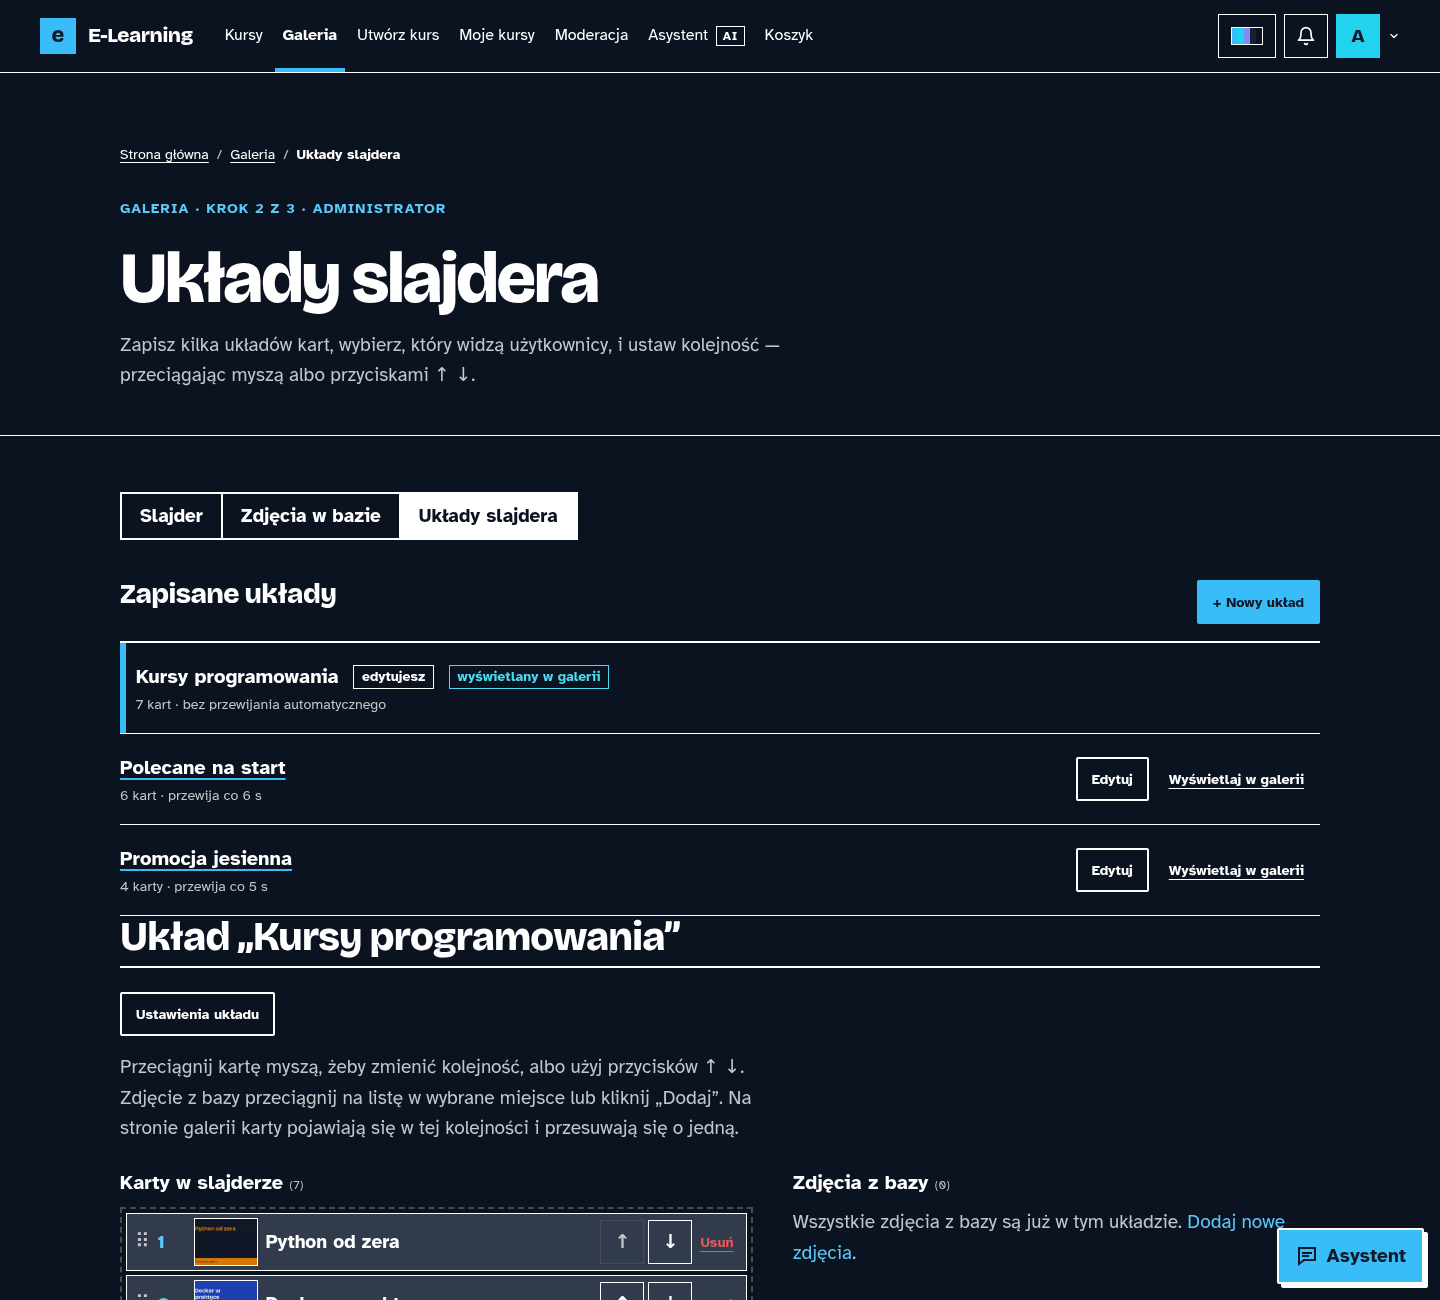
\includegraphics[width=0.94\linewidth,height=0.37\textheight,keepaspectratio]{img/configurator.png}}
\caption{Konfigurator układów slajdera}\label{fig:ui-configurator}
\end{figure}
Lista układów z~oznaczeniem edytowanego i~wyświetlanego; karty przeciągane myszą lub przenoszone przyciskami $\uparrow\downarrow$, obok zdjęcia z~bazy do dodania.


\begin{figure}[H]
\centering
\fcolorbox{rule}{white}{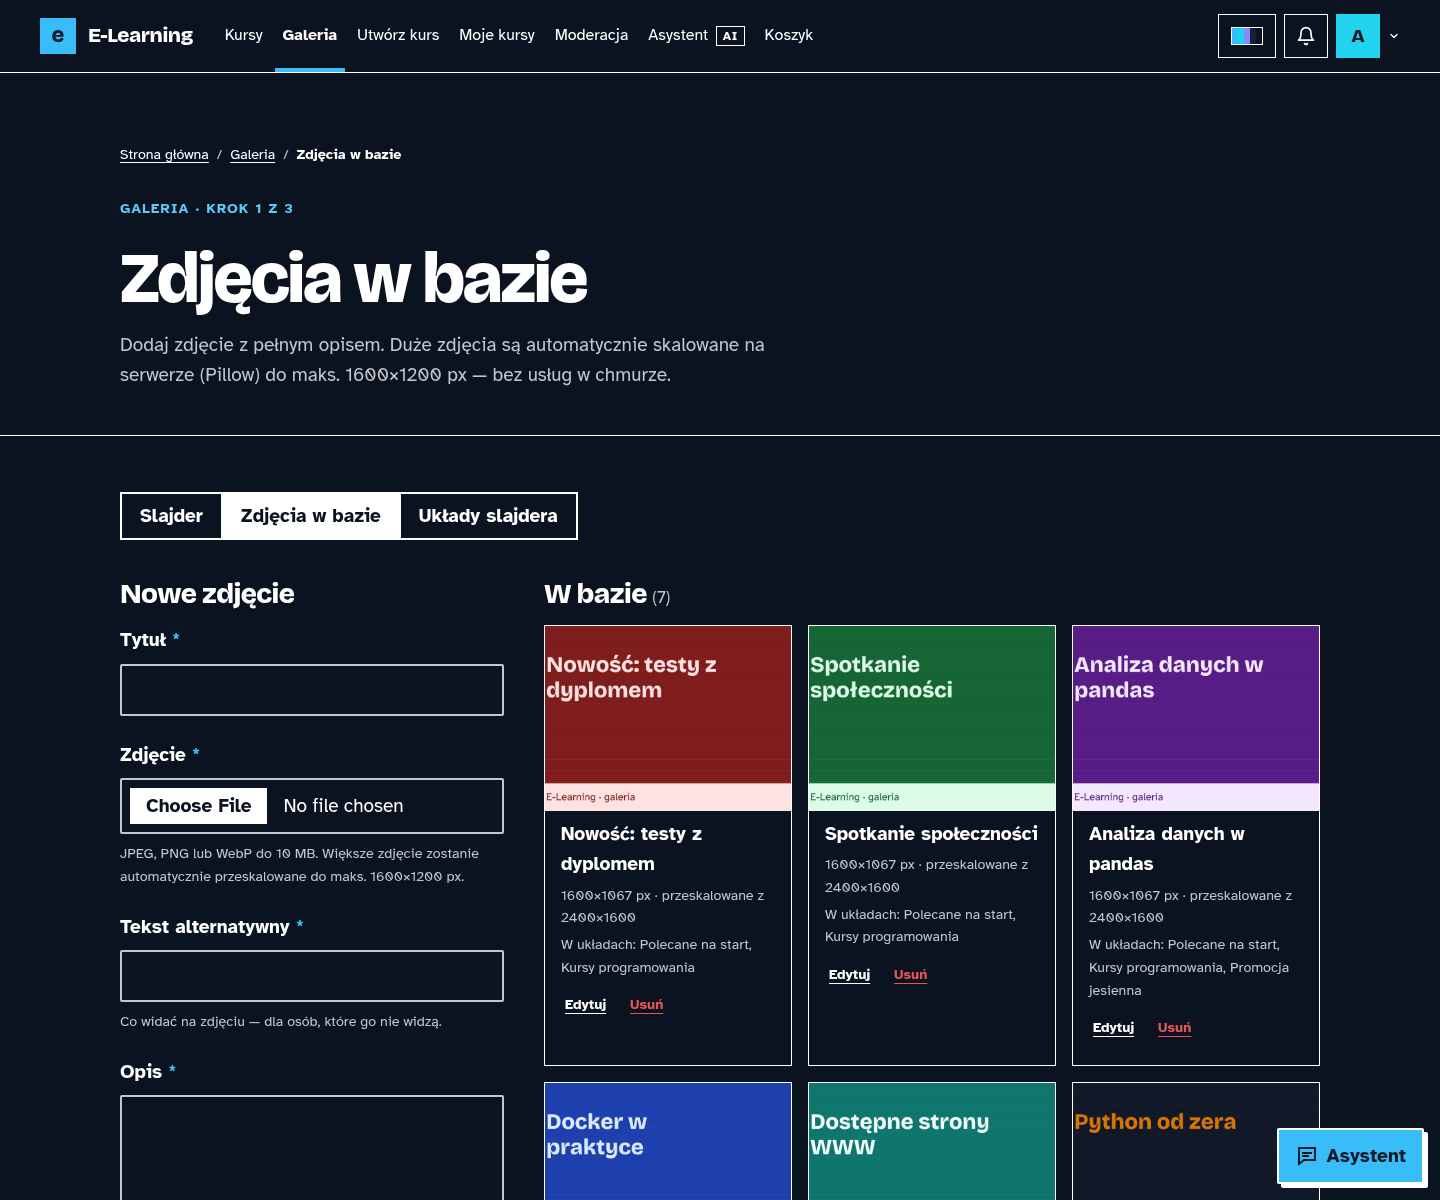
\includegraphics[width=0.94\linewidth,height=0.37\textheight,keepaspectratio]{img/upload.png}}
\caption{Dodawanie zdjęć do galerii}\label{fig:ui-upload}
\end{figure}
Formularz z~wymaganym tekstem alternatywnym i~informacją o~automatycznym skalowaniu; obok baza zdjęć.


\begin{figure}[H]
\centering
\fcolorbox{rule}{white}{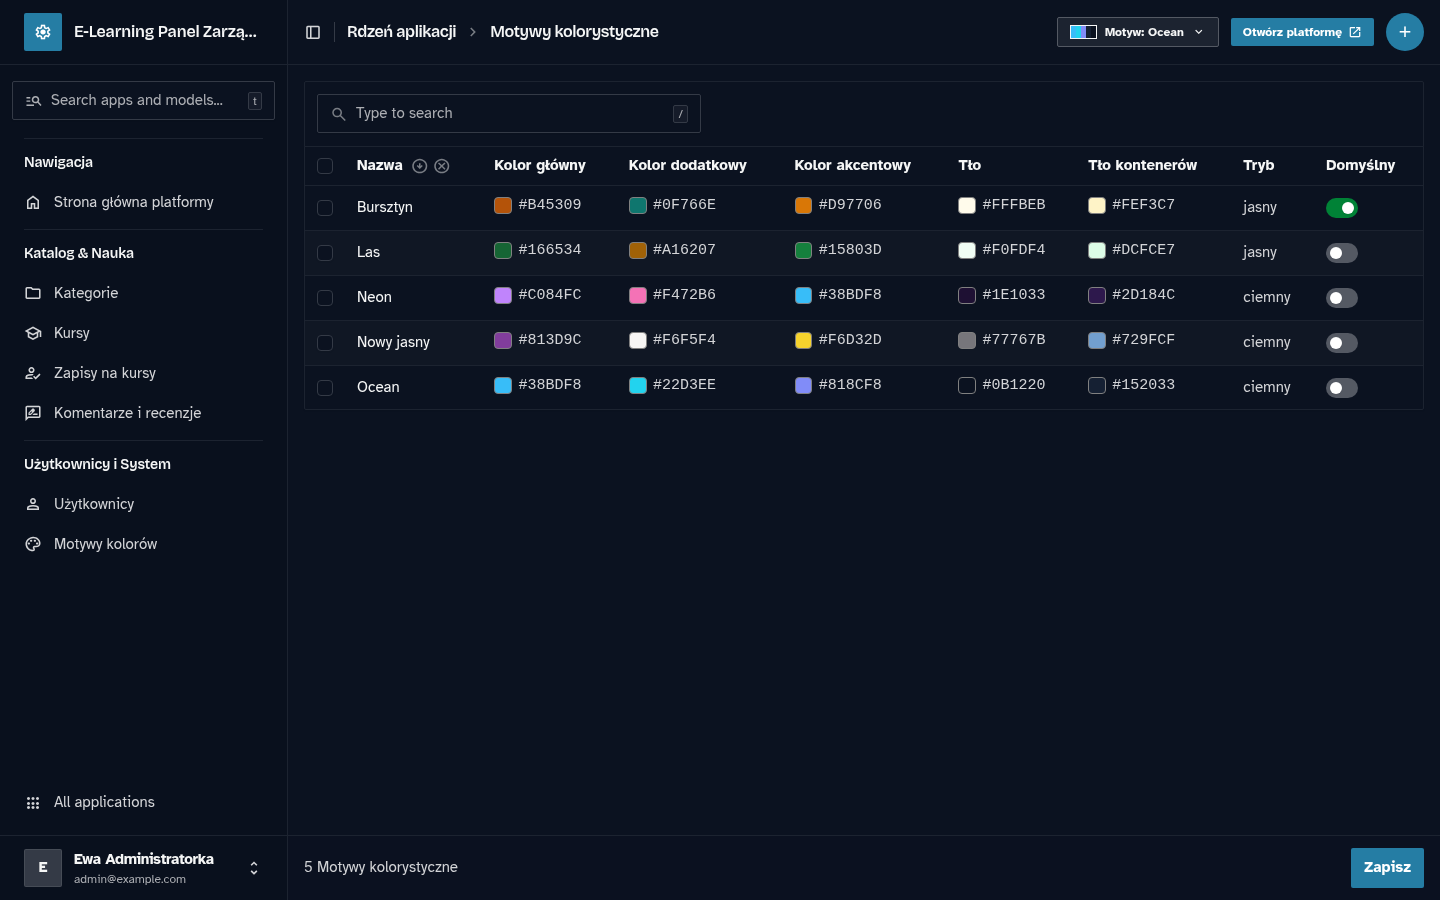
\includegraphics[width=0.94\linewidth,height=0.37\textheight,keepaspectratio]{img/admin_theme.png}}
\caption{Panel administracyjny -- motywy kolorystyczne}\label{fig:ui-admin-theme}
\end{figure}
Panel django-unfold w~kolorach motywu: lista motywów z~pięcioma kolorami, trybem (wyliczonym) i~przełącznikiem motywu domyślnego.


\section{Style uczenia się, ankieta, polecanie, statystyki}
\begin{figure}[H]
\centering
\fcolorbox{rule}{white}{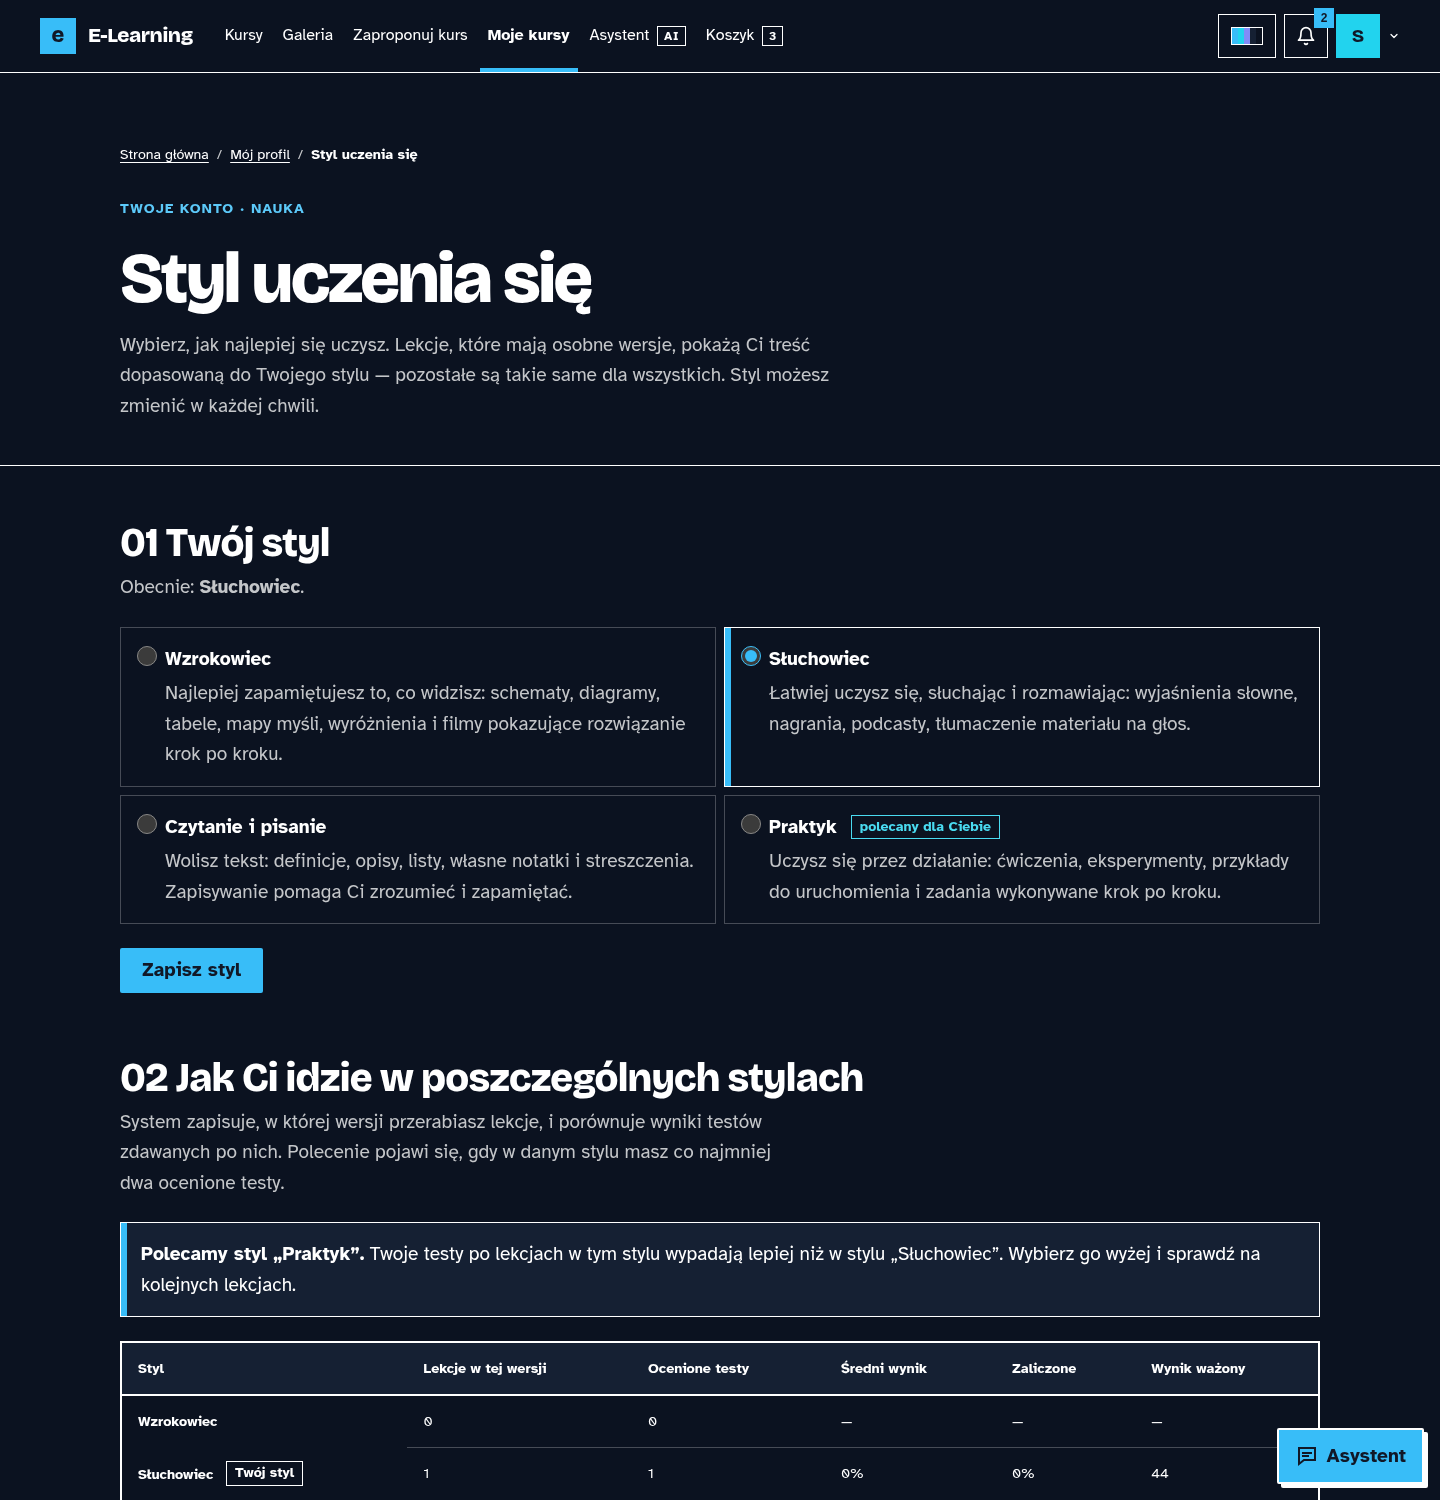
\includegraphics[width=0.94\linewidth,height=0.37\textheight,keepaspectratio]{img/style_student2.png}}
\caption{Strona stylu uczenia się -- uczeń z~rekomendacją zmiany stylu (motyw ciemny)}\label{fig:ui-style}
\end{figure}
Karty wyboru stylu to grupa pól radio w~\code{fieldset}; pod nimi komunikat z~rekomendacją i~tabela wyników w~podziale na style.

\begin{figure}[H]
\centering
\fcolorbox{rule}{white}{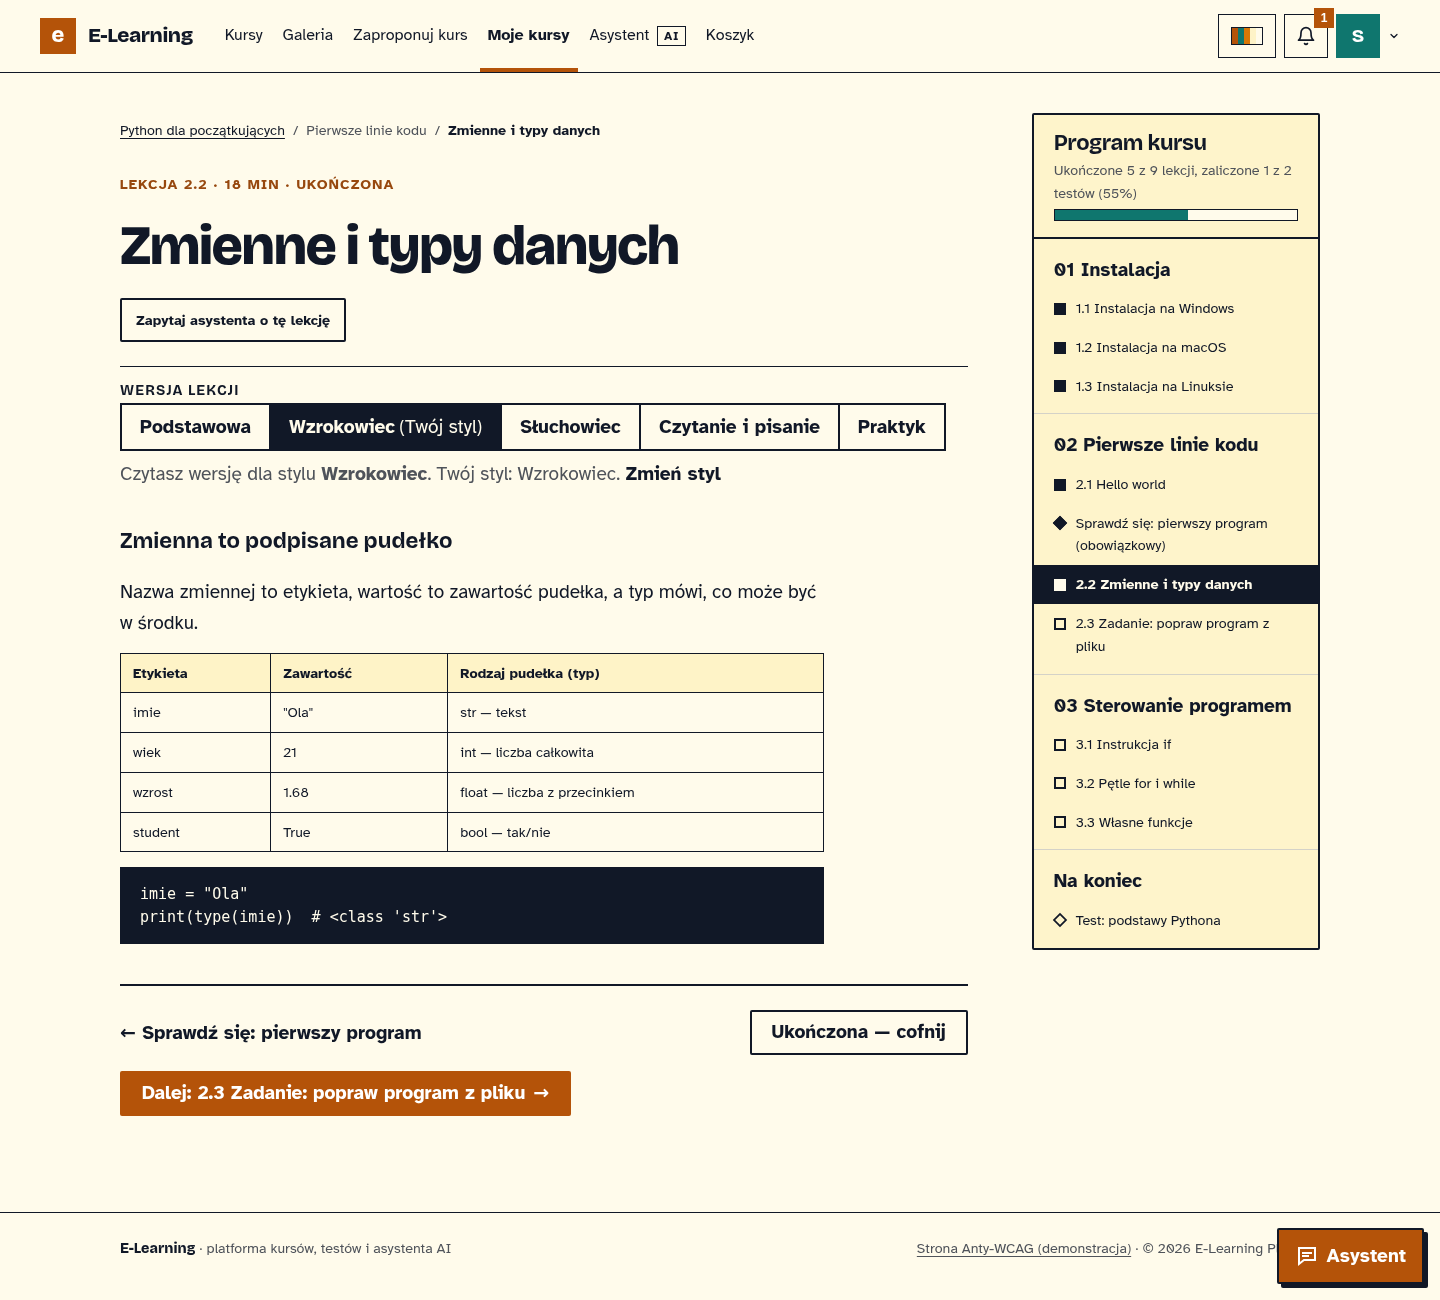
\includegraphics[width=0.94\linewidth,height=0.37\textheight,keepaspectratio]{img/lesson_variant_s1.png}}
\caption{Lekcja w~wersji dla stylu ,,Wzrokowiec'' z~przełącznikiem wersji}\label{fig:ui-variant}
\end{figure}
Przełącznik wersji to nawigacja z~linkami (\code{aria-current} na wyświetlanej wersji); wersja stylu ucznia jest oznaczona ,,(Twój styl)''.

\begin{figure}[H]
\centering
\fcolorbox{rule}{white}{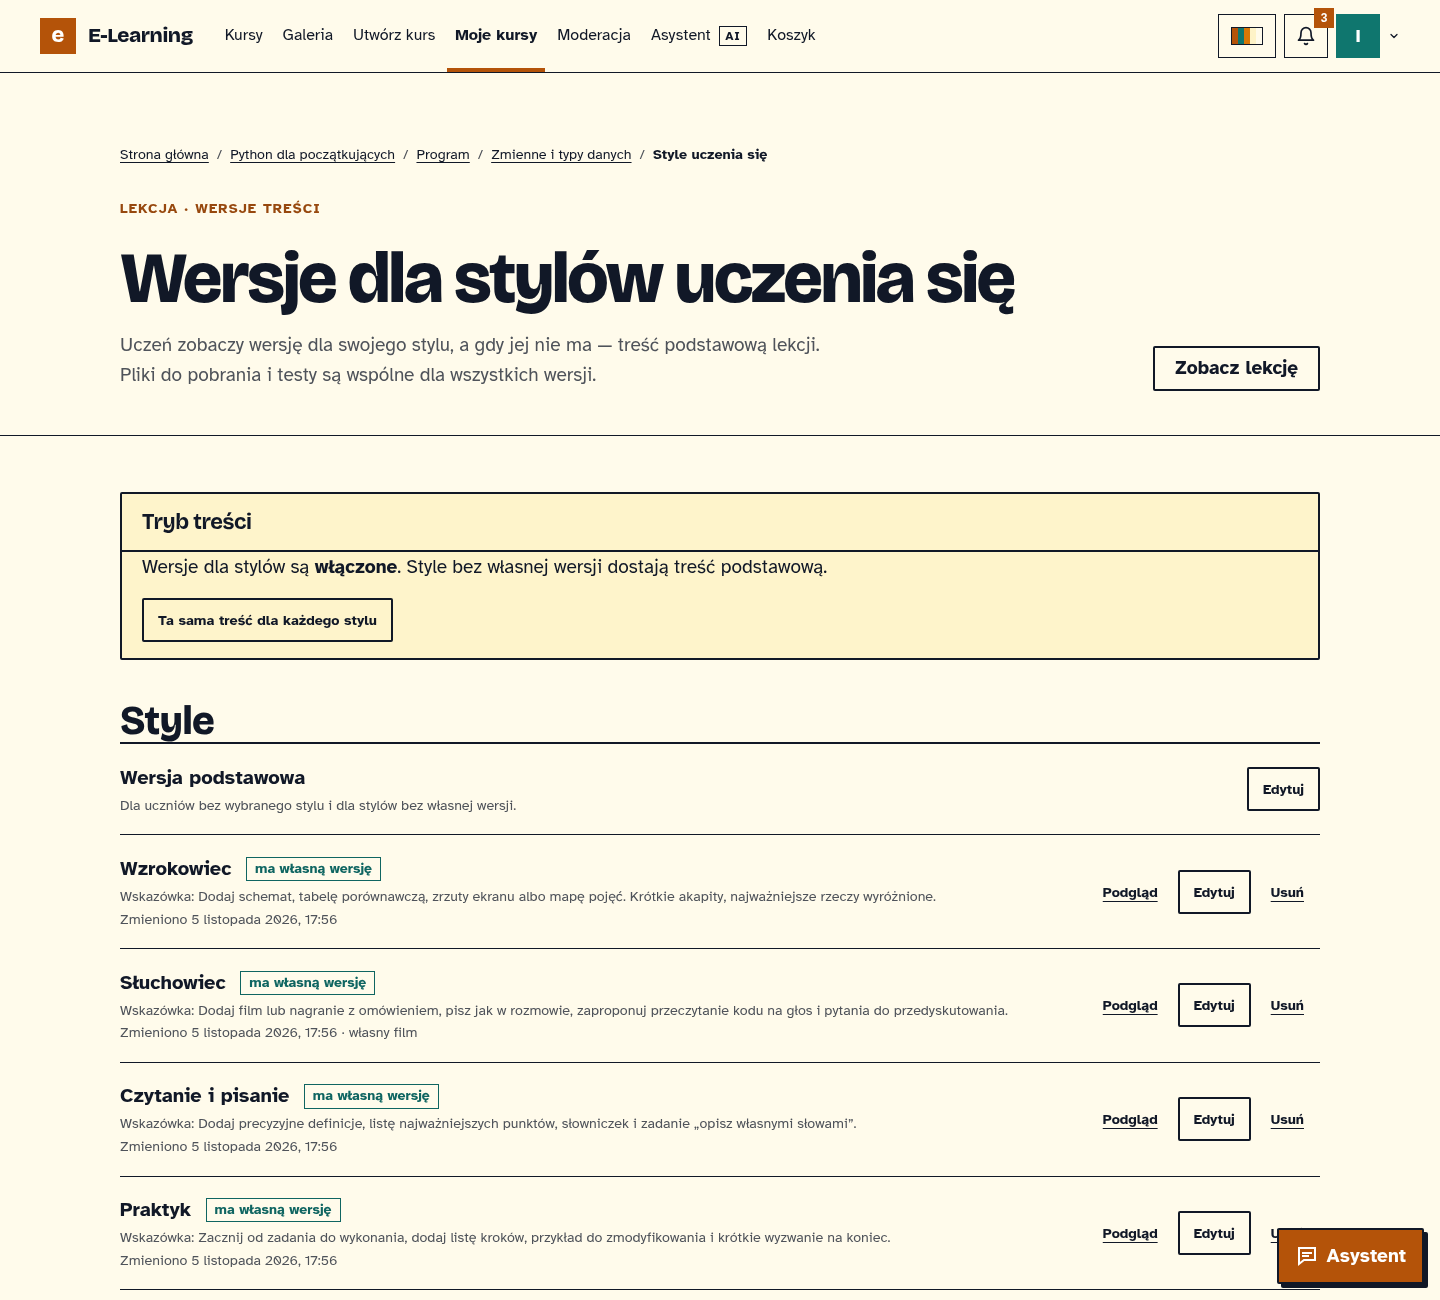
\includegraphics[width=0.94\linewidth,height=0.37\textheight,keepaspectratio]{img/variants_list.png}}
\caption{Autor kursu -- wersje lekcji dla stylów}\label{fig:ui-variants}
\end{figure}
Dla każdego stylu: stan (własna wersja albo treść podstawowa), wskazówka dla autora i~akcje podglądu, edycji oraz usunięcia z~dialogiem potwierdzenia.

\begin{figure}[H]
\centering
\fcolorbox{rule}{white}{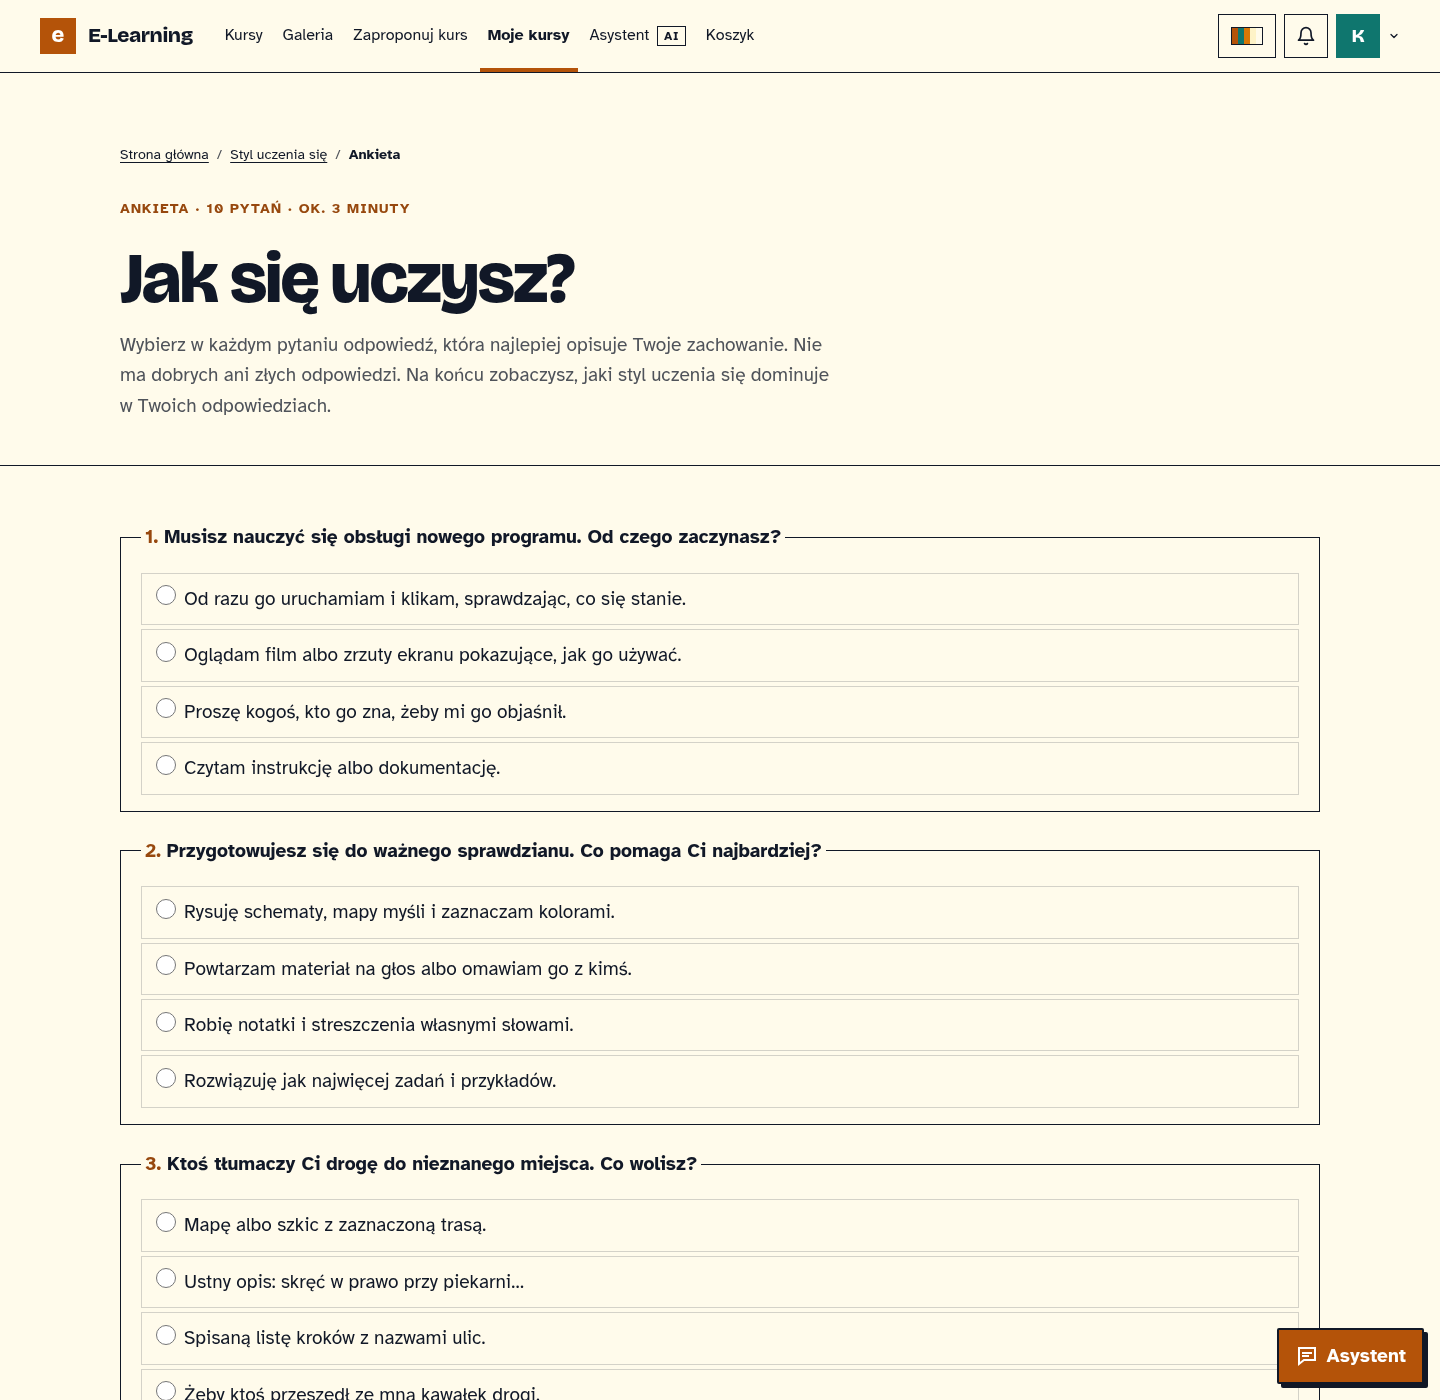
\includegraphics[width=0.94\linewidth,height=0.37\textheight,keepaspectratio]{img/n_survey.png}}
\caption{Ankieta stylu uczenia się}\label{fig:ui-survey}
\end{figure}
Dziesięć pytań sytuacyjnych; każde to grupa pól radio z~legendą, błędy opisane przy pytaniu.

\begin{figure}[H]
\centering
\fcolorbox{rule}{white}{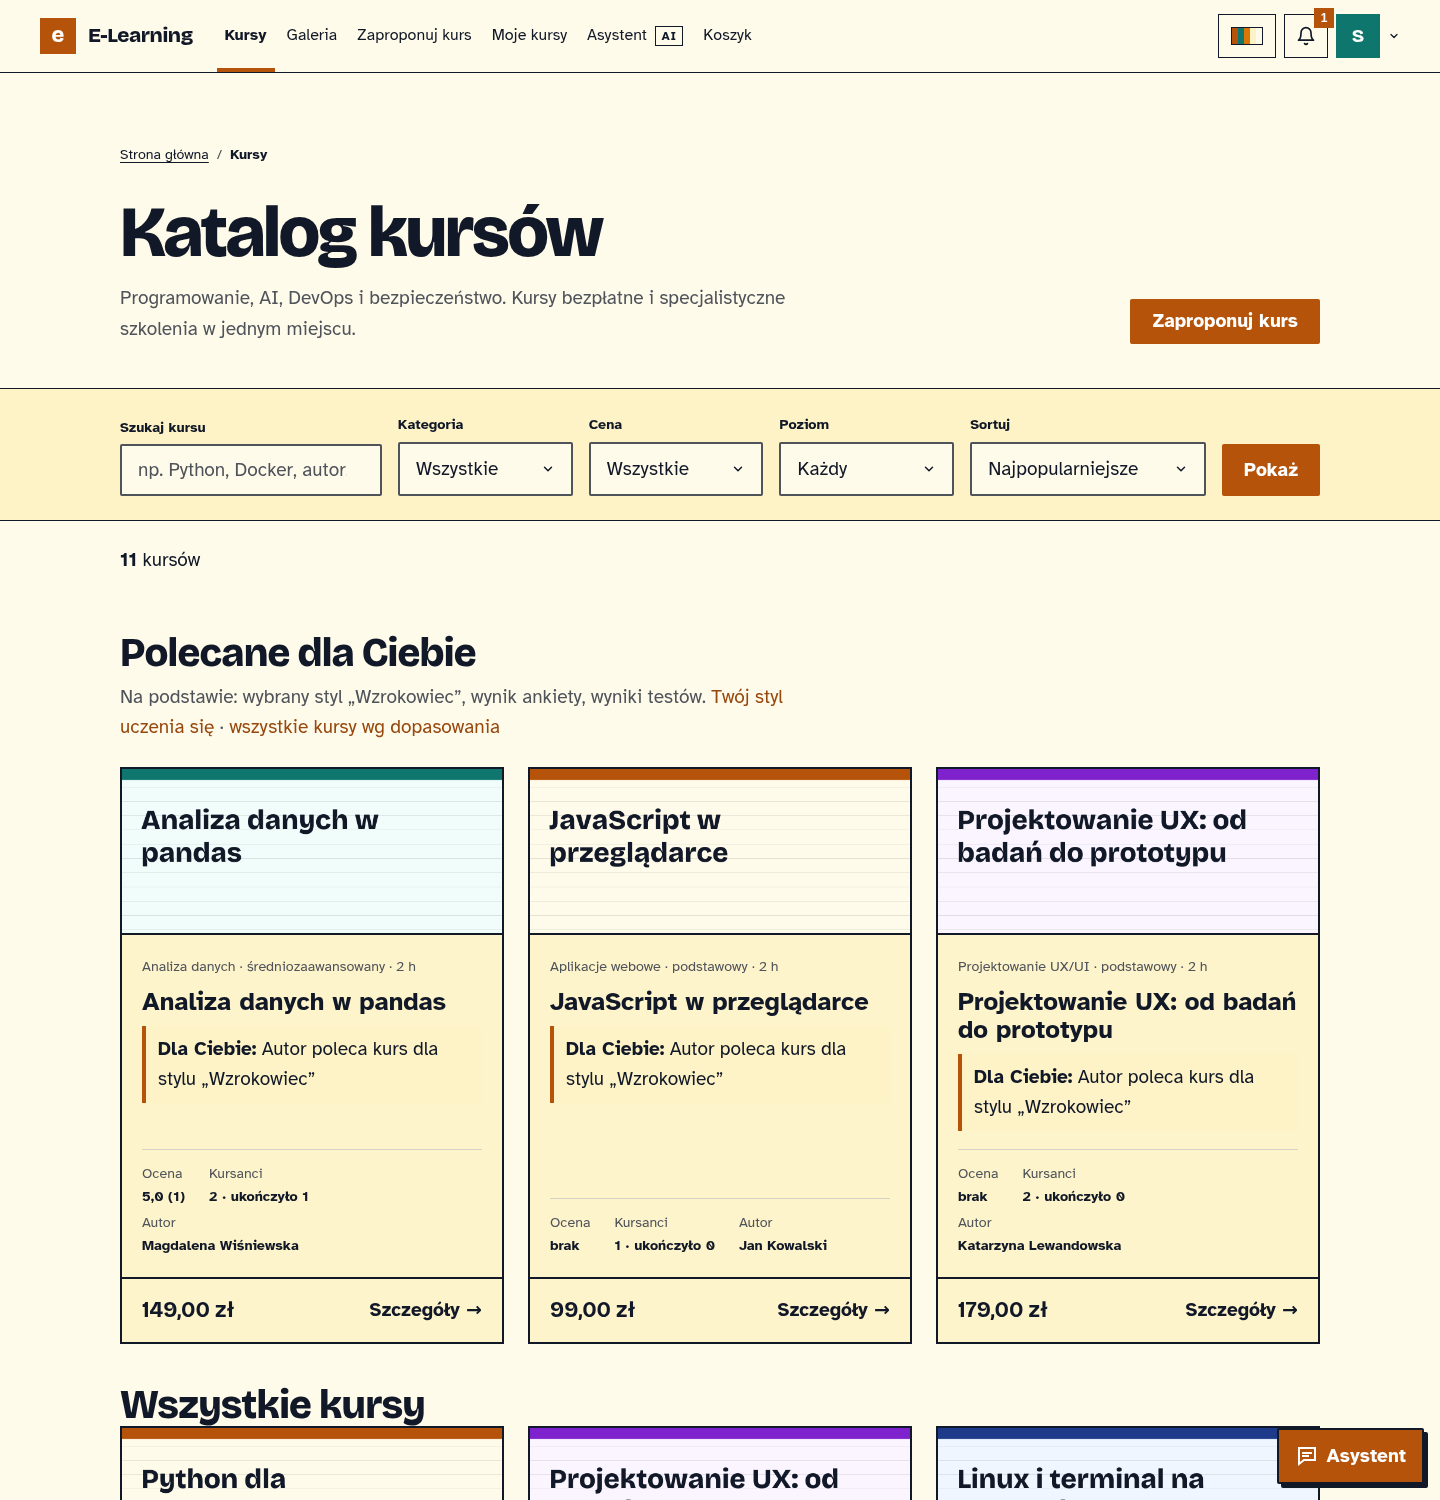
\includegraphics[width=0.94\linewidth,height=0.37\textheight,keepaspectratio]{img/n_catalog.png}}
\caption{Katalog -- sekcja ,,Polecane dla Ciebie''}\label{fig:ui-recommended}
\end{figure}
Nad listą kursów trzy polecenia z~uzasadnieniem (,,Dla Ciebie: …'') i~informacją, z~czego wynika profil; w~sortowaniu opcja ,,Dopasowane do mnie''.

\begin{figure}[H]
\centering
\fcolorbox{rule}{white}{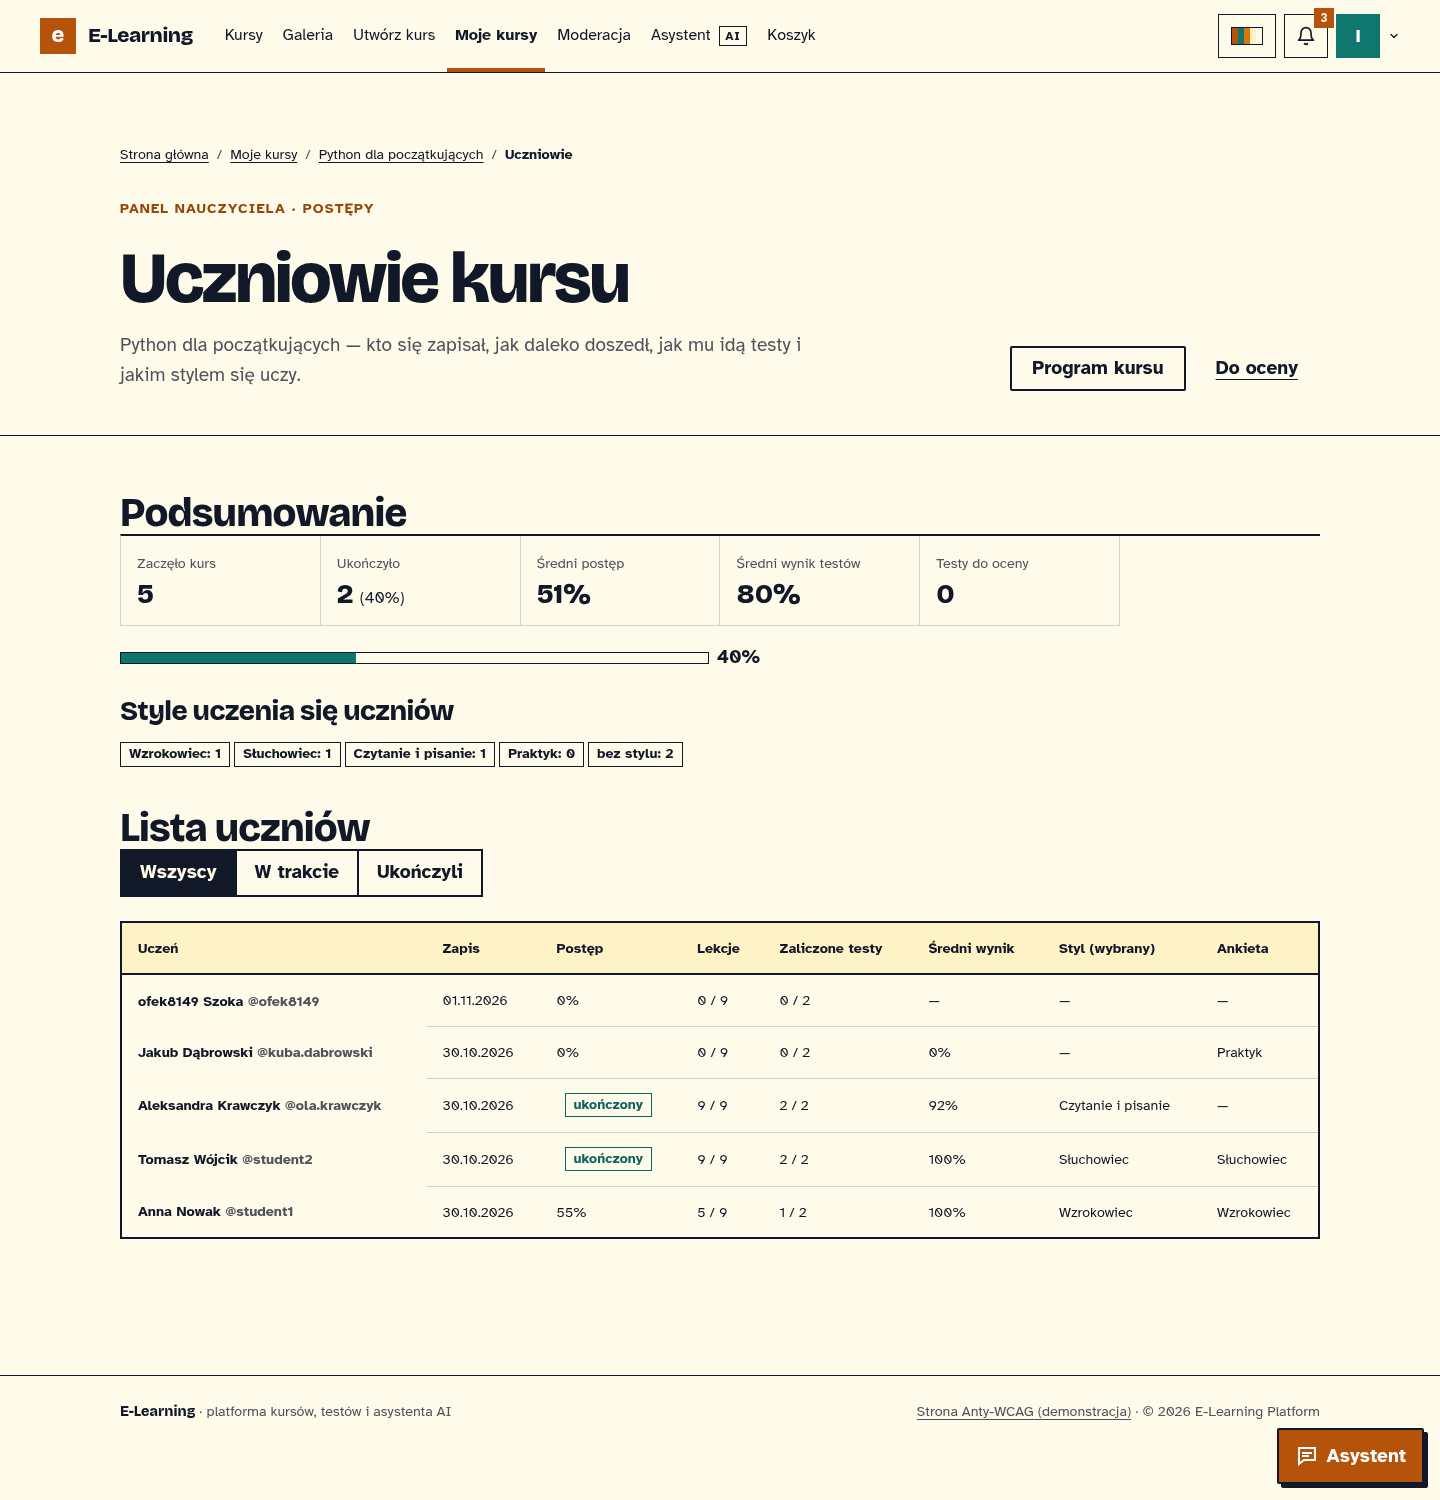
\includegraphics[width=0.94\linewidth,height=0.37\textheight,keepaspectratio]{img/n_students.png}}
\caption{Panel nauczyciela -- uczniowie kursu}\label{fig:ui-students}
\end{figure}
Podsumowanie (zaczęło, ukończyło, procent ukończenia, średni postęp i~wynik), rozkład stylów i~tabela uczniów z~filtrem.

\begin{figure}[H]
\centering
\fcolorbox{rule}{white}{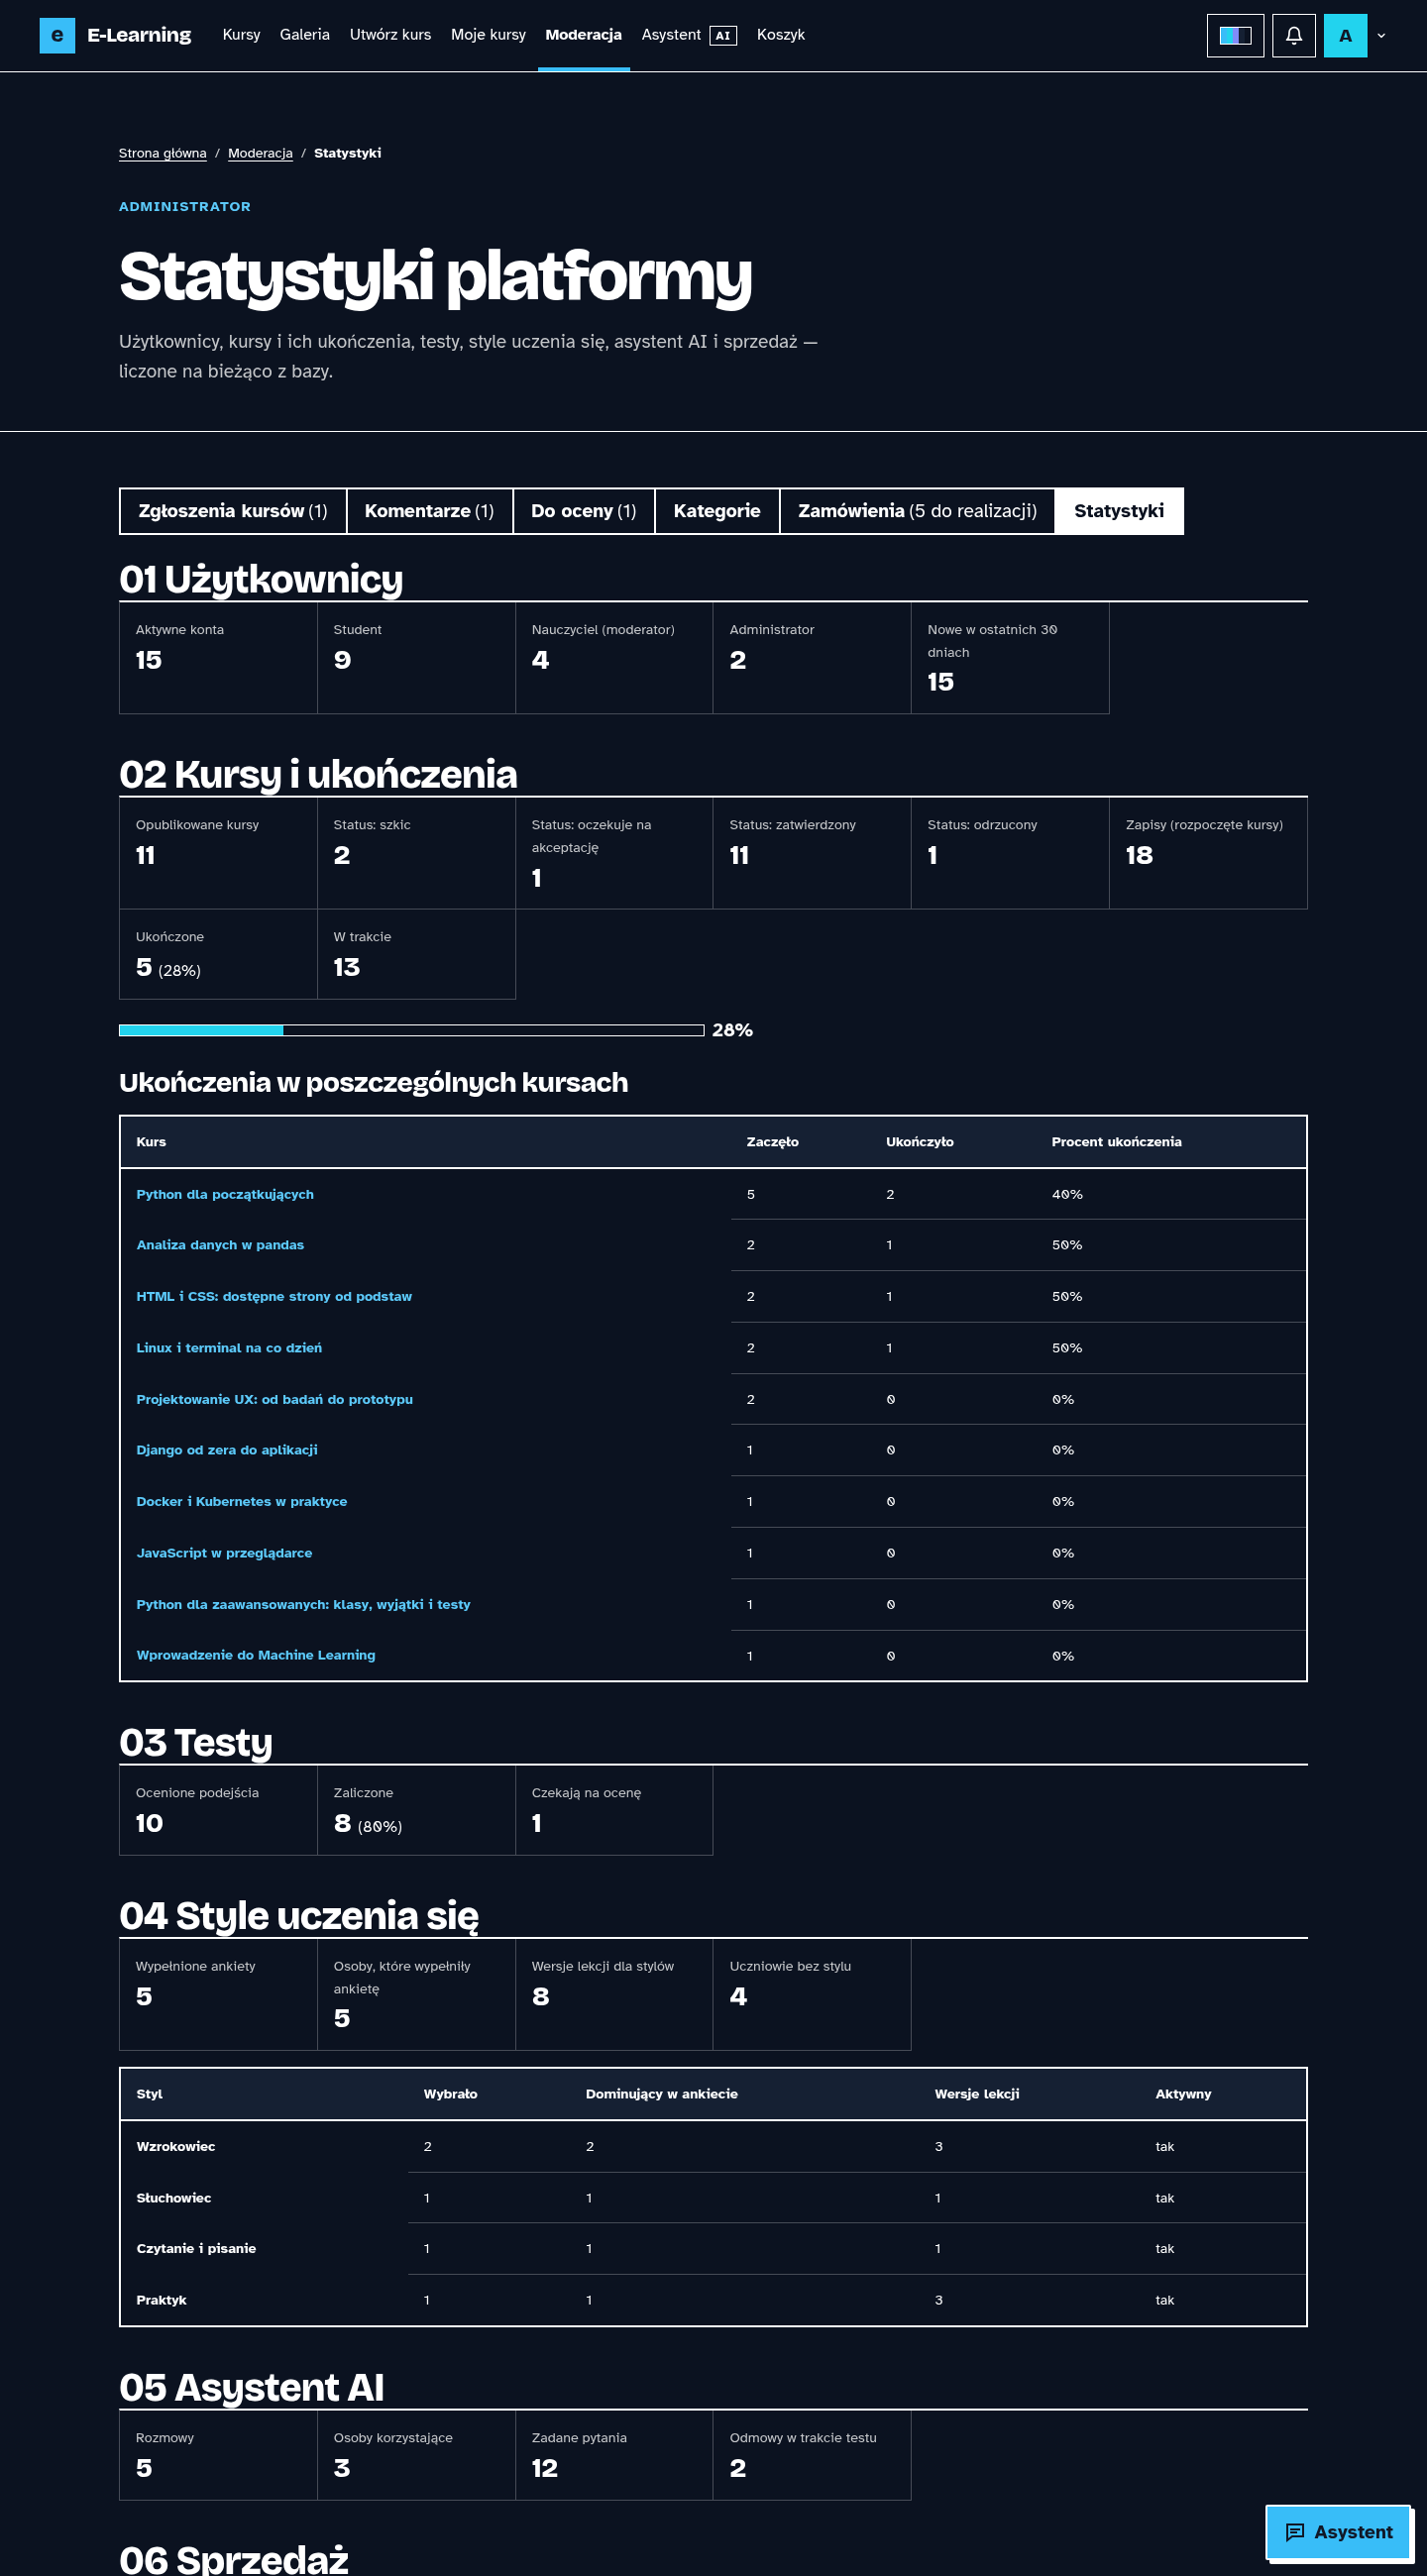
\includegraphics[width=0.94\linewidth,height=0.37\textheight,keepaspectratio]{img/n_stats.png}}
\caption{Statystyki platformy (administrator, motyw ,,Ocean'')}\label{fig:ui-stats}
\end{figure}
Liczby z~bazy w~sześciu obszarach; tabela ukończeń w~każdym kursie z~procentem ukończenia.

\section{Galeria}

\begin{figure}[H]
\centering
\fcolorbox{rule}{white}{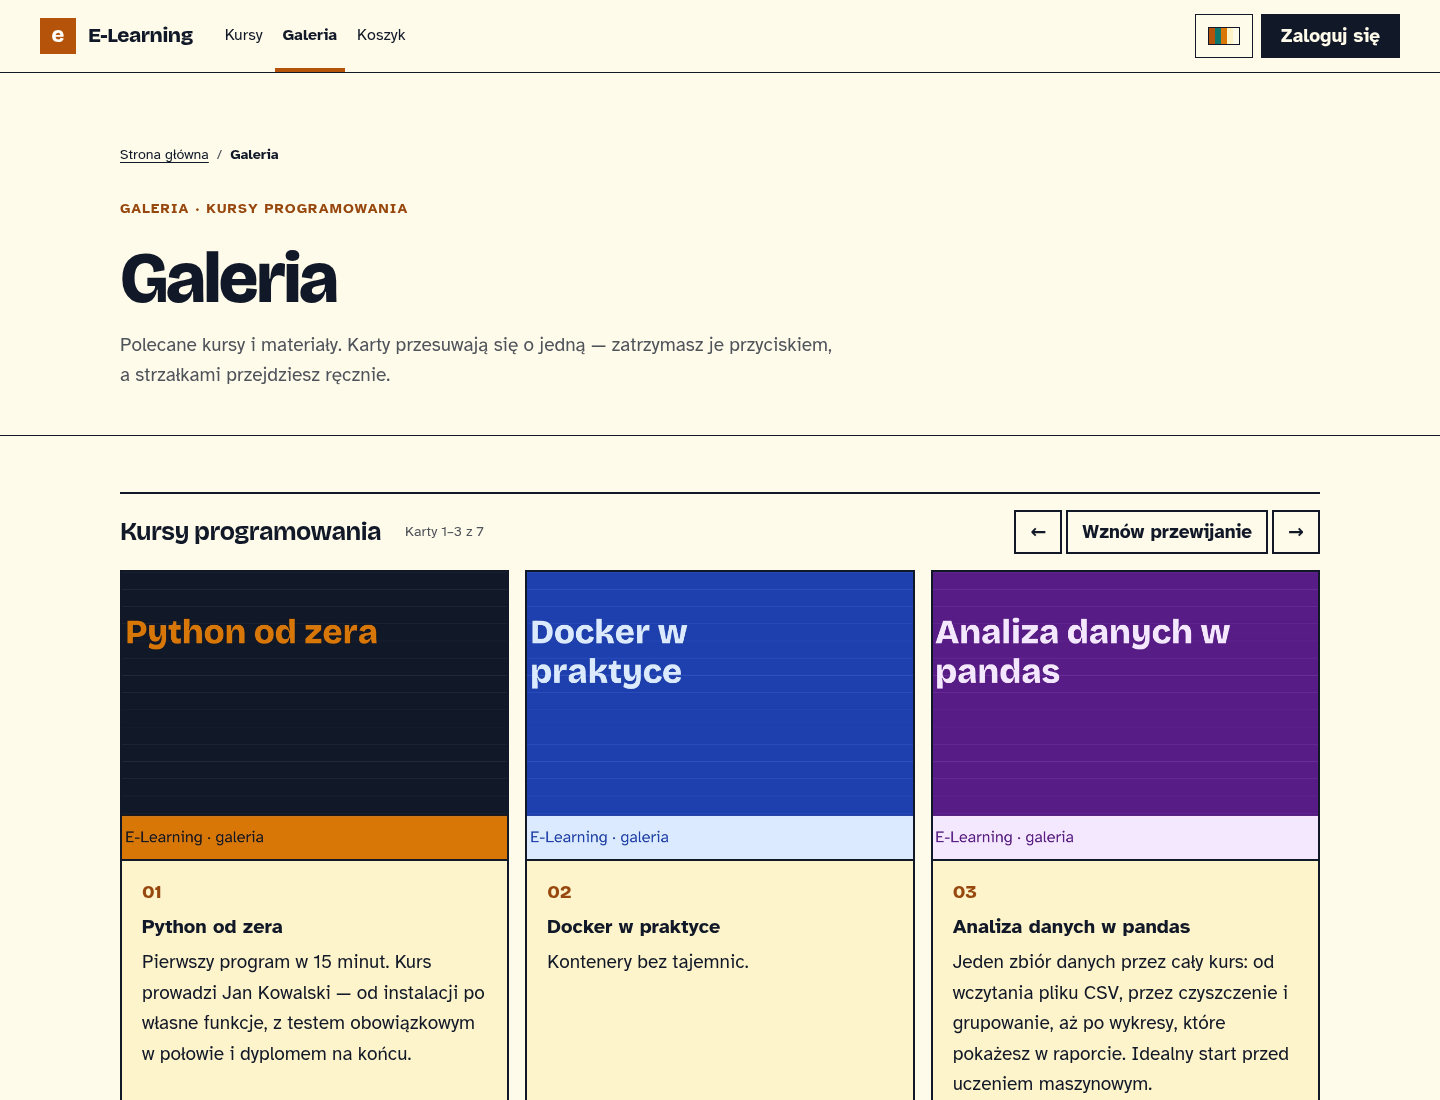
\includegraphics[width=0.94\linewidth,height=0.37\textheight,keepaspectratio]{img/slider.png}}
\caption{Publiczny slajder}\label{fig:ui-slider}
\end{figure}
Trzy karty na komputerze, pełne opisy, przyciski $\leftarrow$, pauza, $\rightarrow$ i~licznik ,,Karty 1--3 z~7''.



